% !Mode:: "TeX:UTF-8"

\chapter{基于梯度自动优化的脑电辨识模型}
情绪和疲劳状态在人的日常生活中扮演着重要的角色。前者能够对人的身心健康和工作效率等产生极大的影响,后者则可能对社会安全产生严重危害。EEG信号作为一种数据载体,可以包含人脑在不同状态下的大量信息,是广泛使用的评估人类心理、生理状态的指标之一。利用EEG信号进行的情绪和疲劳状态辨识,能够有效协助心理健康治疗以及工作疲劳预警。在各种分析方法中,深度学习,尤其是卷积神经网络,作为一种有效提取EEG信号特征的方法,在近年来取得了显著的成果。

虽然深度学习具有自动提取特征和有效分类的优点,但它也面临着网络结构设计困难,需要大量先验知识的问题。自动设计网络结构可以大幅节省专家的时间,因此,神经架构搜索技术应运而生。在本文中,针对EEG信号的时频域特点,对现有基于梯度的NAS算法——PC-DARTS\cite{3-7}进行了针对性的结构改进和优化。

具体来说:(1) 本节在人工设计的针对EEG的高性能网络架构的基础上,设计了一个新颖的CNN架构搜索空间,应用于基于EEG的大脑状态辨识任务。该搜索空间针对EEG特性设计,搜索过程无需从头开始,有效降低了搜索的时间复杂度。(2) 针对EEG通道之间的位置特征,EEG的频域特征以及各个通道的时域特征,提出了双流搜索框架,以提高网络的识别精度。(3) 在PC-DARTS的基础上,设计了自适应算法和早停算法,根据网络拟合情况自动调整模型的复杂度。使得NAS技术在EEG场景中的有效推广成为可能。

本章共引入三个数据集,将所提出架构应用于基于EEG的情绪识别和疲劳驾驶评估任务中。三个数据集包括公开的情绪辨识数据集、公开的疲劳驾驶数据集,以及一组由JS-AINS-40系统采集得到的情绪辨识数据集。结果表明,与现有的方法相比,本文得到的模型架构在这两项任务中都能达到具有竞争力的结果。这一结果不仅验证了所提出算法的性能,还证明了JS-AINS-40系统的可靠性。

\section{基于梯度自动优化的脑电辨识模型}
本节主要从针对不同类型EEG信号的特征提取、所设计算法的基础模型架构以及算法的具体优化框架三个方面展开,对所提出的EEG辨识模型进行了详细描述。
\subsection{特征提取}
EEG是对大脑皮层不同空间位置的测量,它包含多个时间序列。已有工作发现\cite{3-1},EEG信号不仅在频域有很大的差异,还具有明显的空间特征。因此,分析过程可以同时从频域、时域和电极的空间位置开始。为了证明上述特点,进一步对EEG信号进行以下处理。

(1) 差分熵

在深度学习技术出现之前,差分熵(Differential Entropy,DE)是常用于EEG辨识的人工特征\cite{3-2}。基于DE的方法在情感识别任务中取得了显著的效果,被证明是该领域中最有效的人工特征。对一段遵循高斯分布$N\left(\mu, \sigma^2\right)$的时间序列$X$,其DE的计算流程可以如下表述:
\vspace{3mm}
\begin{equation}
\begin{split}
    \label{deqn_ex3_1}
	h(X) &= -\int_{-\infty}^{\infty} \frac{1}{\sqrt{2 \pi \sigma^2}} e^{-\frac{(x-\mu)^2}{2 \sigma^2}} \log \left(\frac{1}{\sqrt{2 \pi \sigma^2}} e^{-\frac{(x-\mu)^2}{2 \sigma^2}}\right) d x\\
    &= \frac{1}{2} \log \left(2 \pi e \sigma^2\right)
\end{split}
\end{equation}
其中$\mu$,$\sigma^2$分别代表高斯分布的均值和方差,$e$为自然常数。

(2) EEG图像

将EEG信号转化为含有空间信息的图像是EEG分析领域的一种常见方法\cite{3-3}。对相应类型的EEG时间序列分别提取其DE特征(情绪EEG数据),进行快速傅里叶变换(Fast Fourier Transform,FFT)(疲劳EEG数据)来提取其频域特征。鉴于DE特征和EEG单一频段内的对数功率谱密度具有等同性\cite{3-10},以及它们在情绪识别和疲劳辨识领域的有效性\cite{3-2,3-30},本章将分别根据DE特征值和FFT的结果生成EEG图像,其具体步骤如下。

首先,为了保留头皮上EEG电极的三维空间分布信息,使用方位等距投影(Azimuthal Equidistant Projection,AEP)\cite{3-4}将电极的三维坐标投影到二维平面。这种方法有效地保留了电极之间的相对位置信息。

其次,应用Clough-Tocher算法\cite{3-5}对每个电极不同频段的DE值或FFT结果,根据二维电极坐标进行插值,并根据电极的数量生成适当大小的图像。在本文中,情绪EEG图像的大小被设定为64×64(公开的情绪辨识数据集)或48×48(JS-AINS-40系统采集得到的情绪辨识数据集),疲劳EEG图像的大小被设定为32×32。

最后,根据不同类型EEG信号的不同特点,对每个包含关键信息的频段都重复这一过程。对于具有$F$个频段的特定EEG信号,这种方法将产生$F$个不同的EEG地形图。$F$个EEG地形图将被合并,形成一个具有$F$通道的图像,作为模型输入的一部分。

\subsection{基础模型架构}
受试者的EEG时间序列将同时在时域和频域中被分割,以作为模型的输入。输入的每个样本由频域的EEG地形图$I$和时域的EEG时间序列$S$共同组成,其中$I \in R^{E \times E}$并且$S \in R^{C \times T}$。$E$代表像素数目,$C$代表EEG电极数,$T$代表每段EEG信号的采样点。在已有研究的基础上\cite{3-6},本章提出双流神经网络作为网络结构搜索的基础框架。双流意味着网络模型由两个具有不同输入模式的分支组成,并且两个分支通过各自相应的候选操作进行针对性构建。本模型的两个分支因其各自的特点被命名为频域流和时域流。图\ref{fig3-1}展示了该网络的框架。

\begin{figure}[!h]
	\centering
	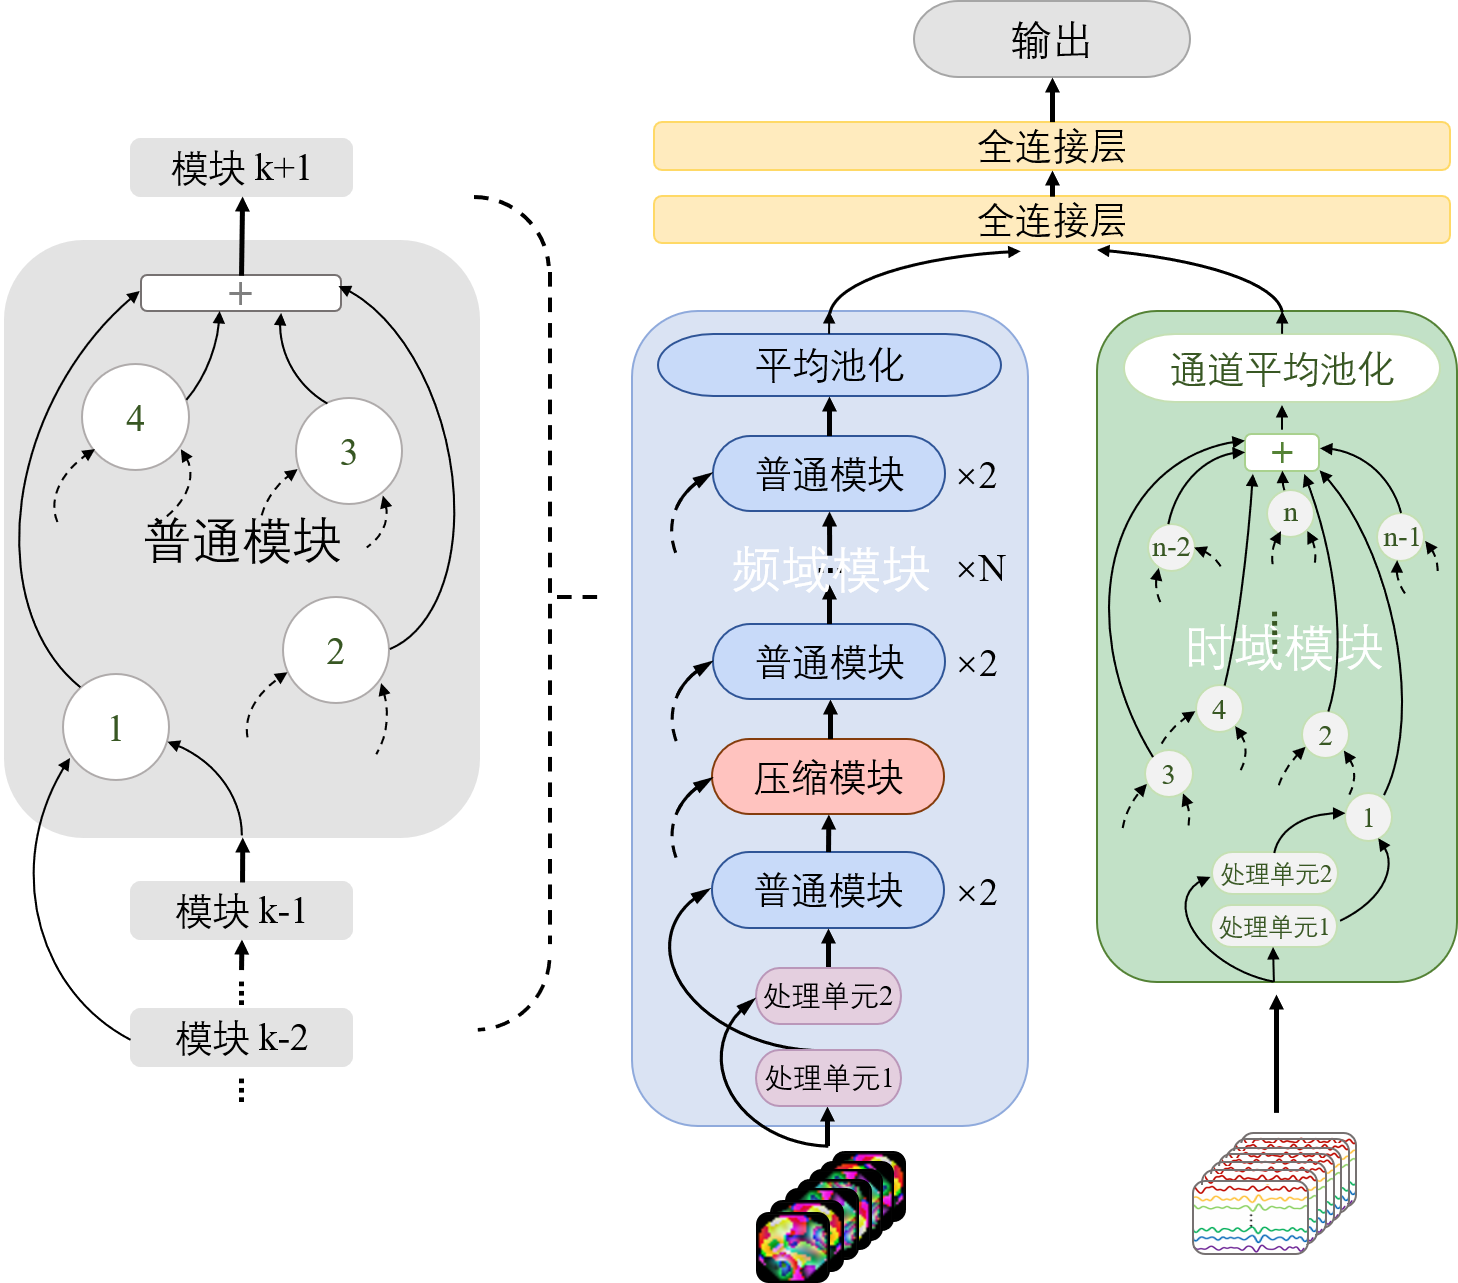
\includegraphics[width=0.55\textheight]{主模型图1.png}
	\caption{双流神经网络框架结构} 
	\label{fig3-1}
\end{figure}

(1) 频域流

将EEG信号转化为图像的相关研究\cite{3-3}验证了电极间相对位置这一信息的重要性,它同时也证明了通道间卷积对EEG特征提取的有效性。借鉴这一领域的先验知识,设计网络框架中的频域流。频域流将EEG图像作为输入,并使用图像识别中常用的扩张卷积(Dilated Convolution)、可分离卷积(Separable Convolution)、最大池化(Maximum Pooling)和平均池化(Average Pooling)作为候选操作来提取EEG图像的空间和频率特征。在图\ref{fig3-1}的左侧是频域流的具体结构和内部连接,以及频域流内部普通模块的结构。频域流的设计继承自PC-DARTS,其框架结构由普通模块和压缩模块堆叠而成。普通模块与压缩模块的内部结构相同,但后者通过引入步长(Stride)为2的候选操作,实现了对特征图大小的压缩(压缩模块的原理在3.1.3优化框架一节中详细介绍)。压缩模块的存在保证了模型能够在深度增大时,时刻保持压缩特征,扩张感受野以及提取全局特征的能力,为模型架构的变化提供性能支撑。EEG图像输入时,频域流首先使用处理单元1与处理单元2对输入的EEG图像进行3×3卷积运算,形成第一个普通模块的两个输入。普通模块内部节点上的虚线代表两个候选操作。频域流中$N$被设置为4。

(2) 时域流

已有研究\cite{3-8}引入了一个名为巧合筛分卷积神经网络(Coincidence-Filtering-based CNN,CF-CNN)的模型,它只对EEG信号的每个通道进行两次时间卷积(Temporal Convolution)和一次通道平均池化(Channel Average Pooling)。该模型有效地利用了巧合筛分的思想,成功地提取了EEG信号的时间依赖性以及EEG电极通道的具体特征。它的优越性已经在疲劳判别和情绪识别数据集中得到了证明。在CF-CNN模型的基础上,选择时间卷积和通道平均池化操作来提取与通道相关的特征,完成时域流的构建。在图\ref{fig3-1}的右侧,展示了时域流的独特结构以及它所包含的时域模块的内部连接方式。时域流包含一个时域模块,时域模块内部首先通过两个处理单元对输入的时域信号进行1×1卷积运算,为第一个节点生成两个输入。连接到内部节点的虚线也代表两个任意的候选操作。在本章中,时域模块内部的$n$被设定为11。

在网络的最后,两个流的输出通过两个全连接层结合起来,完成EEG信号的识别。然而,上述模型的有效性高度依赖于架构设计和超参数选择。因此,引入网络结构搜索算法,在一个广阔的搜索空间上进行结构搭建,以寻找EEG信号的特定模式。

\subsection{优化框架}
为了以最小的计算资源消耗快速演化网络结构,使用基于梯度的网络结构搜索算法作为参考。其中PC-DARTS作为这一领域中的经典框架,在对CIFAR-10数据集的图像进行分类时,成功的将模型架构搜索时间减少到了2.4小时以内。因此,本章的研究将以该方法为基础进行展开。

(1) 网络结构搜索空间

PC-DARTS的多分支结构有助于建立复杂的网络框架,并在图像识别任务中取得了瞩目的成果。因此,本章将在模型中保留这一结构,并将其应用于基于EEG的模型结构搜索中。本节在3.1.2节基础模型架构的基础上,为两个流建立不同的搜索空间。整体来看,模型的搜索空间中包含有三种不同的模块(普通模块、压缩模块和时域模块)。

在频域流中,由于模型的输入是EEG图像,其数据结构与RGB图像相似,因此本章保留了PC-DARTS中的所有原有候选操作,并在此基础上搜索最适用于该流的模块结构,其中包括3×3大小的最大池化、3×3大小的平均池化、3×3大小、5×5大小的可分离卷积、3×3大小、5×5大小的扩张卷积、直接连接以及无连接。所有卷积操作的卷积核数量被设定为16。

在普通模块和压缩模块内部,设置了四个节点(不包括两个输入节点和一个输出节点)。节点的概念继承自PC-DARTS,它本质上代表了对网络中的张量的连接操作。这些张量来自前位的节点或模块,它们的输出经过一组特定的操作后到达当前节点。节点这一特殊概念的引入有利于网络结构的设计和变更。每个节点只可以接收其前向方向上任意两个节点(或者模块)的输出。模块内所有节点的输出将被串联成为模块的输出。

从普通模块和压缩模块外部来看,根据已有研究中的模型规模\cite{3-3},频域流中堆积的模块的初始个数被设置为11。堆积模块的策略也将遵循PC-DARTS的设计——网络由两个普通模块与一个压缩模块交替构建。压缩模块是一个特殊的模块,其引入的目的是减小通过网络的特征图的大小。为了达到这个目的,与压缩模块的输入节点相邻的所有节点上的候选操作都将被设置步长为2。每个模块将前面两个模块的输出作为输入。频域流的最终输出将通过一个平均池化层传递给全连接层。在搜索过程中,模型将不断调整频域流内的模块堆叠数量,而频域流模块内部的节点数量将一直保持不变。

在时域流中,参考CF-CNN的设计,将网络构建为只包含一个模块(时域模块)的结构。最初,时域模块将包含11个内部节点(不包括两个输入节点和一个通道平均池化节点)。在这11个节点之间,有1×1、1×3、1×5、1×7、1×9、1×11大小的时域卷积、直接连接和无连接作为候选操作。所有卷积操作的卷积核个数被设定为32。这些操作确保了时域流将优先提取与通道相关的时间信息。与频域流一样,每个节点可以从其前向方向上的任意两个节点处接收输出。在搜索过程中,模型将不断调整时域流内的节点数量,而时域模块的数量将一直保持不变。

(2) PC-DARTS在EEG上的改进

当模型规模设置过大或训练集容量过小时,PC-DARTS在网络结构搜索过程中会随着训练迭代次数的增加而更易倾向于选择弱参数操作(如直接连接、最大池化等),造成网络结构的崩塌现象\cite{3-9}。这种现象产生的根源在于网络中不同模块的前后堆叠。网络输入端的模块接触到的是最纯净的信息,而整个网络后端的模块接触到的是已经提取过的抽象特征(随着网络结构的加深,这个问题将愈加明显),因此后端的模块将倾向于直接传递抽象特征,即使用直接连接操作,以获得更好的分辨能力。由于模型内部的同种模块之间结构共享,这一问题将会扩散至整个网络,使得模型最终发生崩塌。

同时,由于PC-DARTS以与网络权重相同的方式将操作权重转换为可微调的对象,并将架构搜索过程转换为双层优化问题:
\begin{equation}
\label{deqn_ex32}
\begin{array}{cl}\min _\alpha & \mathcal{L}_{\text {val }}\left(w^*(\alpha), \alpha\right) \\ 
\text { s.t. } & w^*(\alpha)=\operatorname{argmin}_w \mathcal{L}_{\text {train }}(w, \alpha)\end{array}
\end{equation}
这使得网络权重和操作权重的优化形成一个竞争过程。网络权重$w$因为具有更多的可学习参数,对交替训练过程中损失的变化相对鲁棒,因此在竞争中对操作权重$\alpha$具有一定的优势。$\alpha$为了在竞争中获得胜利,将会变得更倾向于选择弱参数操作,这增大了模型崩塌的概率。

此外,PC-DARTS为减少性能消耗,使用了部分通道连接(Partial-Channel-Connections)的方法:
\begin{equation}
    \label{deqn_ex33}
f_{i, j}^{\mathrm{PC}}\left(\mathbf{x}_i ; \mathbf{S}_{i, j}\right)= \sum_{o \in \mathcal{O}} \frac{\exp \left\{\alpha_{i, j}^0\right\}}{\sum_{o^{\prime} \in \mathcal{O}} \exp \left\{\alpha_{i, j}^{o^{\prime}}\right\}} \cdot o\left(\mathbf{S}_{i, j} * \mathbf{x}_i\right)+\left(1-\mathbf{S}_{i, j}\right)^* \mathbf{x}_i
\end{equation}
其中$\mathbf{S}_{i, j}$代表了随机采样掩码。这一方法使得每次网络结构更新时,只有少数通道被更新,而其余部分保持不变。这进一步促使网络选择弱参数操作,加剧了网络结构崩塌的风险。尽管PC-DARTS设计了边缘正则化方法:
\begin{equation}
    \label{deqn_ex34}
\mathbf{x}_j^{\mathrm{PC}}=\sum_{i<j} \frac{\exp \left\{\beta_{i, j}\right\}}{\sum_{i<j} \exp \left\{\beta_{i, j}\right\}} \cdot f_{i, j}\left(\mathbf{x}_i\right)
\end{equation}
为每一个模块中节点的输入引入了一个参数$\beta$,$\beta_{i, j}$代表了节点$i$,$j$之间的边缘正则化权重,能够一定程度上减弱上述影响。

但边缘正则化的存在有时并不能保证网络的最终搜索结果不会崩塌(特别是在数据量较少的EEG数据集上)。因此,本章在训练过程中引入了层数自适应机制和早停机制:
在NAS搜索过程完成后,如果模块内被选为直接连接的边数达到25\%,则认为搜索已经崩塌,网络将自动降低模型复杂度——减少堆叠模块的数量(针对频域流)或模块内的节点数量(针对时域流),开始新一轮搜索。如果在停止训练时,模型的训练精度仍然不能稳定在85\%以上,那么认为应该增加模型的复杂度(增加堆叠模块的数量或模块内的节点数量)。

在NAS过程中,当操作权重$\alpha$在一段时间内(一定数量的epochs,在本章中设置为10)保持稳定时,就可以停止NAS进程。


\section{实验描述}
在本章中,基于EEG的情绪辨识公开数据集、疲劳驾驶检测公开数据集以及JS-AINS-40采集的情绪辨识数据集将被分别使用,验证所提出模型的有效性。
\subsection{情绪辨识公开数据集}
(1) 数据集描述

在情感识别领域,上海交通大学的情感数据集(SEED)在众多研究中被广泛使用\cite{3-2}。SEED数据集包含了15个受试者(Subject)的EEG信号,这些信号是通过观看15个情绪电影片段收集的。其中有三种类型的情绪,包括高兴、中性和悲伤,每个电影片段大约持续4分钟。每名被试总共包含三个时段(Session),每个时段中均进行15次观影试验。受试者的EEG信号由62个脑电极以1000 Hz的采样率完成记录,这些信号用0 Hz-75 Hz的带通滤波器进行了预处理。之后,采集者将数据降采样至200 Hz。在此基础上,本章将EEG信号沿时间方向划分为一系列不重叠的1秒数据段。此外,挑选了十二个电极的EEG信号作为时域流的输入,即FT7、FT8、T7、T8、C5、C6、TP7、TP8、CP5、CP6、P7和P8,因为研究表明它们在情绪识别中起着重要作用\cite{3-11}。

同时,SEED中所有62个通道的数据被用作频域流的输入,以保留EEG电极之间的空间位置信息。数据DE特征的提取已经在SEED数据集中完成,本章分别提取每个1秒数据段对应的DE特征作为频域流的输入。对于每个1秒数据段,首先使用零填充(Zero Padding)将DE特征扩展到64个通道,之后对其进行归一化处理,即每个被试的数据将减去其平均值并除以其标准差。然后,DE特征的五个频段:$\delta$频段、$\theta$频段、$\alpha$频段、$\beta$频段和$\gamma$频段将被分别转换为相应的EEG图像,将其合并即获得频域流的五通道EEG图像输入。由于不同情绪视频的长度不一致,捕获的情绪EEG信号的长度也不一样。为了保证不同类别数据量的平衡性以及情绪唤醒的有效性,统一选择每段数据的最后185秒和其对应的DE特征作为模型的输入。

(2) 分类模型以及性能度量

为了评估所提出框架的跨被试情绪分类性能,采用留一法(Leave-One-Subject-Out,LOSO)进行验证实验。在本章情况下,这种方法的核心是将测试被试的所有数据从训练数据中剔除,以验证模型是否提取到了关于情绪的通用性特征\cite{3-13}。在每次LOSO实验中,将选择一名被试者的数据作为测试数据,其余被试者的数据被用作训练数据。这个过程将自动重复,直到每名受试者的数据都作为测试集被模型验证过一次。

根据分类结果,本章引入了一些常用的分类指标来评估网络模型的整体性能,包括精度(Precision,PR)、F1分数(F1-score,F1)\cite{3-14}、宏观平均F1分数(Macro-averaging F1-score,MF1)、准确率(Accuracy,ACC)以及来自所有情感类别的接收者操作特征(Receiver-Operating-Characteristic,ROC)曲线的平均曲线下面积(Area Under the Curve,AUC)。这些指标的计算公式如下:

\begin{equation}
    \label{deqn_ex35}
T P R_i=\frac{T P_i}{T P_i+F P_i}
\end{equation}

\begin{equation}
    \label{deqn_ex36}
R E_i=\frac{T P_i}{T P_i+F N_i}
\end{equation}

\begin{equation}
    \label{deqn_ex37}
F 1_i=\frac{2 P R_i \times R E_i}{P R_i+R E_i}
\end{equation}

\begin{equation}
    \label{deqn_ex38}
M F 1=\frac{\sum_i^C F 1_i}{C}
\end{equation}

\begin{equation}
    \label{deqn_ex39}
A C C=\frac{\sum_i^C T P_i}{N}
\end{equation}

\begin{equation}
    \label{deqn_ex310}
A U C=\frac{1}{C_C^2} \times \sum_{\substack{1 \leq j<C-1 \\ 2<k \leq C j<k}}\left[\frac{\sum_l^{N_j+N_k}\left(S_p>S_n\right)+0.5 \times \sum_l^{N_j+N_l}\left(S_p=S_n\right)}{\left(N_{j P}+N_{k P}\right) \times\left(N_{j N}+N_{k N}\right)}\right]
\end{equation}

\vspace{5mm}


其中$T P_i$是类别$i$中真正例样本的个数(True Positive Samples),$F P_i$是类别$i$中假正例样本的个数(False Positive Samples),$F N_i$是类别$i$中假负例样本的个数(False Negative Samples),$C$代表了样本类别数,$N$是测试样本总数,$N_i$是类别$i$中的样本个数,$N_{i P} / N_{i N}$是类别$i$中的正例与负例样本数之比,$S_p$与$S_n$是类别$j$和$k$组成的集合的Wilcoxon-Mann-Witney测试\cite{3-15}分数。

(3) 训练参数

本章模型将SGD优化器与学习率余弦退火算法结合使用,在网络结构搜索阶段最小化模型损失。由于较大的学习率有助于双层优化过程找到更好的架构,因此SGD优化器中参数设置为:学习率0.1、动量0.9、权重衰减0.0003以及batch size 64。搜索过程中dropout概率保持为0.3。根据双层优化过程的性质,将操作权重的学习率设置为0.0006,操作权重衰减率设置为0.001。

训练集数据将被随机分为两个大小相同的子集,分别用于网络权重优化和操作权重优化。由于网络模型在搜索过程中同时优化了超网络中所有候选操作的权重,最终的最优架构不一定具备当前数据的最佳网络权重,因此需要对最优架构进行再训练。

在再训练阶段,利用Adam优化器将网络的损失降到最低。此时学习率被设置为0.02,动量被设置为0.9,权重衰减被设置为0.0012,batch size被设置为64,dropout概率被设置为0.4。再训练阶段无需进行网络结构变动,只需对网络权重进行调整,因此使用较小的学习率寻找权重最优值。

\subsection{疲劳驾驶检测公开数据集}

(1) 数据集描述

本文使用的疲劳驾驶检测公开数据集为Cao等人采集的数据集\cite{3-16}。该数据集收集了27名22-28岁的志愿者的EEG数据。实验使用了32通道的有线脑电极帽来记录EEG信号,其中包括30个EEG电极和2个参考电极。采集时,EEG信号被放大并以500 Hz的采样率进行数字化(在使用中本章进一步将数据降采样至250 Hz)。所有的EEG信号都使用了带通滤波器(1 Hz-50 Hz的有限脉冲响应(Finite Impulse Response,FIR)滤波器)和伪影抑制(Artifact Rejection)来进行预处理。

本数据集的实验模拟了夜间四车道高速公路上的驾驶环境,要求受试者将汽车保持在车道中央巡航。该实验的设计是为了模拟一种非理想的道路状况,它将触发汽车以相等的概率向第三条车道的右侧或左侧进行漂移。每个车道偏离事件包括四个标记:基线期(Baseline Period)、漂移开始(Onset of Drift)、反应开始(Onset of Response)和事件结束(The End of Event)。偏移事件发生前所有30个通道的3秒EEG数据将被进行FFT变换,并提取其$\theta$频带、$\alpha$频带和$\beta$频带。这三个频段被分别插值为32×32大小的图片后,共同构成EEG图像,并作为频域流的输入。


此外,本文只使用Fcz、Tp7、Cp3和Oz通道的EEG时间数据作为时域流的输入,因为研究发现这四个通道在检测驾驶员疲劳方面有着重要作用\cite{3-17}。与上一节一样,每名受试者的数据都进行了归一化操作。

(2) 标签获取

由于原始数据没有提供标签来确定每段EEG是否处于疲劳状态,因此需要进行人工标注。

受试者的反应时间(Response Time,RT)在本章被提取出来作为衡量受试者是否处于疲劳状态的指标。RT是指在模拟驾驶过程中发生汽车漂移与受试者做出纠正反应之间的时间间隔。首先,从当前事件中提取的反应时间被称为局部RT,它代表受试者的短期疲劳状态。在当前事件之前的90秒内所有事件的平均反应时间被称为全局RT,代表受试者的长期疲劳状态。将在整个90分钟的实验中获得的所有局部RT从小到大进行排序,并将第$Z$个RT作为实验的警戒RT($Z$等于某个被试的样本总数乘以5\%),它代表受试者在实验期间清醒状态下的反应速度。当偏移事件的局部RT和全局RT都小于警戒RT的1.5倍时,认为此时被试是清醒的;当偏移事件的局部RT和全局RT都大于警戒RT的2.5倍时,认为被试此时处于疲劳状态。介于两者之间的部分没有被分类,因为这可能归因于其他未知的过程,例如,受试者在进行思想游荡\cite{3-18}。
\newpage
(3) 训练参数

为了使每名受试者的疲劳和清醒事件保持平衡,本章删除了六个不符合条件的受试者。从数据集的角度来看,最终选择的21名受试者共包含11,772个不同类别EEG样本,其中疲劳状态的数量为6,054,清醒状态的数量为5,718,二者基本处于平衡状态。

同样,LOSO交叉验证法被用来验证模型的性能。引入的评价指标与之前的一致。模型架构搜索和再训练阶段的超参数与情感识别任务中的超参数相一致。




\subsection{JS-AINS-40系统情绪辨识数据集}
为验证JS-AINS-40的实际使用效果,设计相应的EEG情绪实验。本章使用JS-AINS-40系统和搭载配套上位机软件的计算机(带有音响)作为实验器材。
在本次实验中获得的数据集即JS-EM Dataset,实验的详细内容如下所述。

(1) 被试与实验内容

本次实验共选取了13名年龄在20-30岁之间受试者(8名男性,5名女性),这些受试者均身体健康,无视力、听觉障碍及大脑相关疾病。所有被试在实验开始前均进行了一段时间的情绪平复,以保证实验开始时情绪能够被正常唤起。同时,向所有受试者介绍了实验的具体流程,以保证实验的顺利进行。13名受试者中有5人从未参加过任何EEG实验,其他人则有过相关实验经历。本实验经过了天津医科大学总医院的伦理委员会的审查,并签署了知情同意书。

本章实验引入了三类不同电影的片段,分别对应高兴、悲伤与中性三种不同的感情。每段影片均经过精心挑选与编辑,能够创造连贯的情感,并可以最大程度唤起受试者的相应情绪。被试需要在相对独立,没有外部环境干扰的房间中独自观看影片,以保证EEG数据的有效性。具体内容如表\ref{tab3-1}所示。

\begin{table*}[!h]
\caption{电影片段具体信息}  \label{tab3-1}
\centering
\wuhao{
    \begin{threeparttable}
    \setlength{\tabcolsep}{5mm}{
        \begin{tabular}{cccc}
            \toprule
            编号 &电影片段来源 &情绪类型 &片段时常\\
            \midrule
            1   &武林外传        &高兴   &9分35秒\\
            2   &憨豆先生1       &高兴   &8分45秒\\
            3   &憨豆先生2       &高兴   &9分10秒\\
            4   &亲爱的          &悲伤   &8分30秒\\
            5   &七号房的礼物     &悲伤   &9分55秒\\
            6   &舐犊情深        &悲伤   &9分20秒\\
            7   &航拍中国(第一季) &中性   &9分40秒\\
            8   &航拍中国(第二季) &中性   &9分50秒\\
            9   &蓝色星球(第一季) &中性   &10分05秒\\
            \bottomrule
        \end{tabular}
        }
    \end{threeparttable}
    }
\end{table*}

每个片段播放结束后,被试都会获得一段情绪平复时间(时长因被试特点而进行调整),以保证每次实验开始时被试均处于中性状态。在情绪平复时间内,被试会被要求填写调查问卷,以获取被试对于实验设计的意见。

(2) 实验流程

实验过程中,屏幕上会全程提示受试者接下来将要进行的实验步骤,保证受试者不会受到外界干扰。实验的具体流程如下所示:1) 受试者稳定情绪,并了解实验相关流程,签署实验同意书;2) 准备阶段,屏幕上提示受试者保持专注,给与受试者十秒钟时间进入状态;3) 情绪唤起阶段,程序随机挑选三类影片中的一段进行播放;4) 情绪平复阶段,观影结束,受试者填写问卷,并平复情绪。
\begin{figure}[!h]
	\centering
	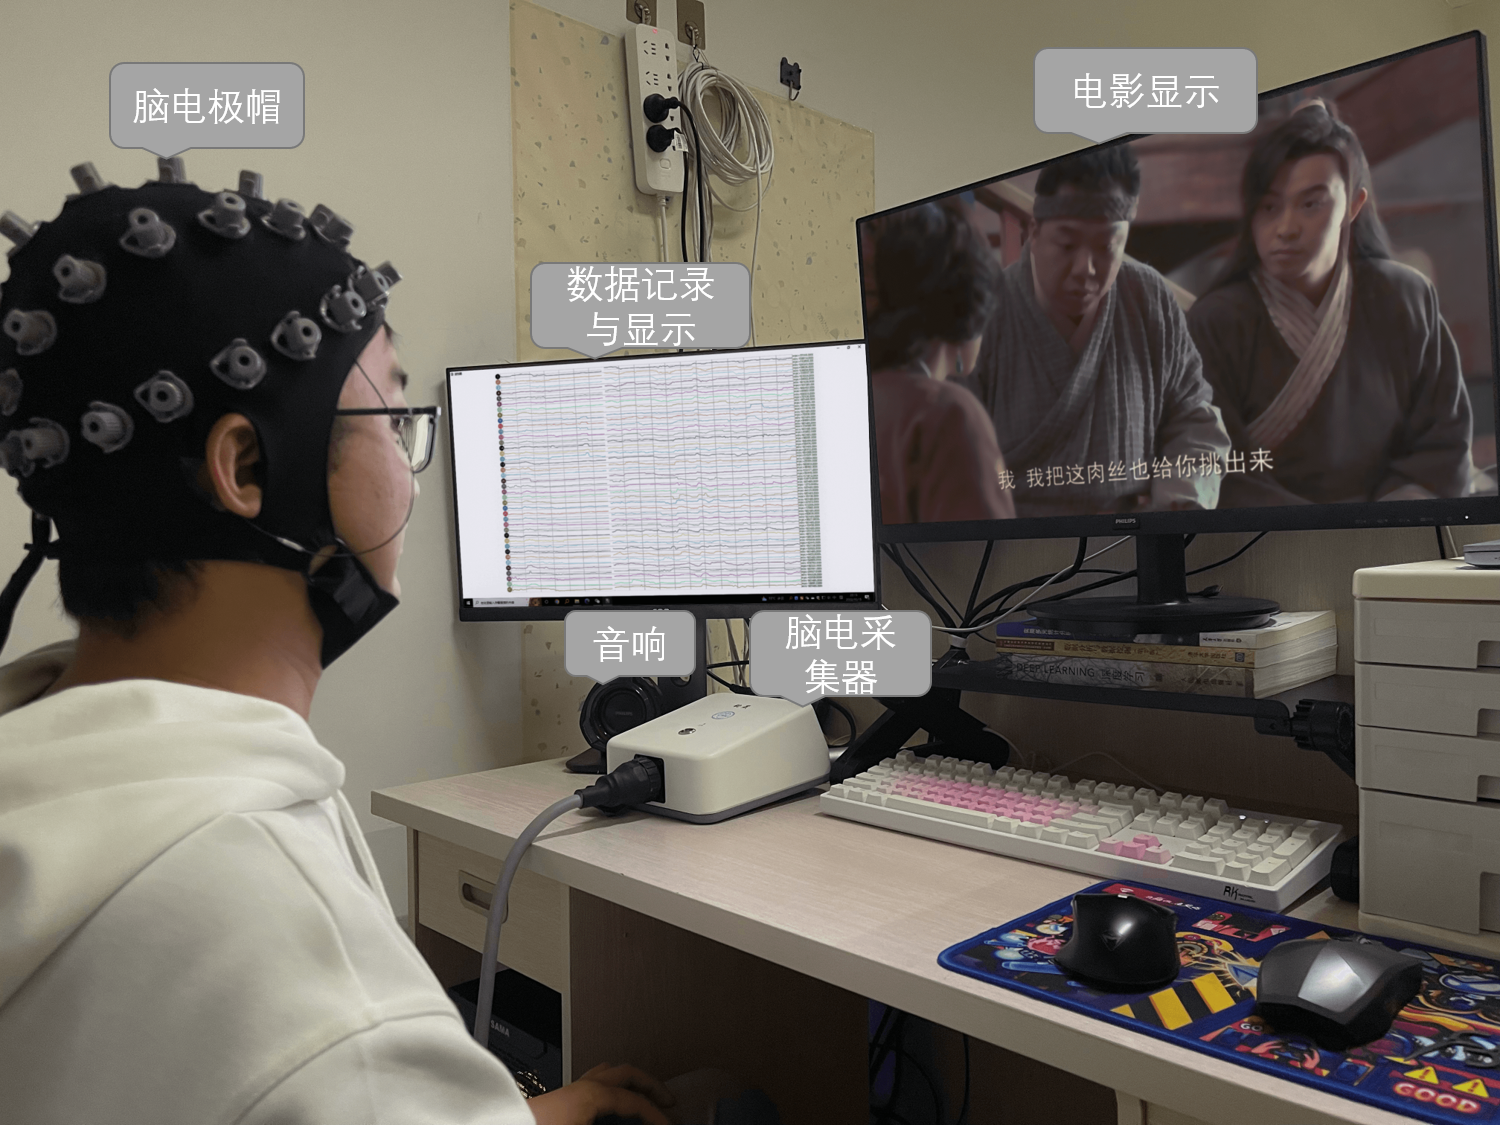
\includegraphics[width=0.44\textheight]{情绪实验.png}
	\caption{情绪实验场景图} 
	\label{fig3-2}
\end{figure}

当第一遍流程结束后,实验将会从阶段2) 准备阶段,重新开始,直至完成18次实验。18次实验中将会包含高兴、悲伤与中性三种电影片段各6次,其出现顺序由电脑随机决定。实验场景如图\ref{fig3-2}所示。

(3) 数据预处理

上述数据以1000 Hz的采样率在50 Hz工频陷波下进行采集。采集后,使用1 Hz-60 Hz的带通滤波器对数据进行滤波,以减小噪声干扰。为降低运算复杂度,将数据从1000 Hz降采样至250 Hz。此后,使用独立分量分析(Independent Component Analysis,ICA)\cite{4-29}来消除伪迹和眼电信号的干扰。

为了保证不同类别数据量的平衡性以及情绪唤醒的有效性,统一选择每段数据的最后360秒,并将其切片为1秒数据
段。全部40个通道的1秒时序信号将作为时域流的输入。对于频域流输入,首先提取1秒数据段的DE特征(频带与SEED中一致),并使用零填充将DE特征扩展到48个通道。之后对其进行归一化处理,即每个被试的数据将减去其平均值并除以其标准差。每个频带的DE特征将被插值为48×48大小的图片,合并后作为EEG图像输入频域流。

(4) 训练参数

LOSO交叉验证法被用来评估模型的性能,同时这里也引入了与之前数据集相同的评价指标。模型架构搜索和再训练阶段的超参数与SEED数据集所设置的超参数保持一致。

\section{结果与讨论}

从搜索中得到的模型结构完成再训练后,就可以被应用在测试数据集上检验模型性能。所有受试者的平均辨识准确率将作为模型性能的评判标准,并与其他基于脑电的辨识算法进行比较。当不同的被试作为测试集时,NAS算法将搜索得到不同的最优网络架构,带来高昂的时间开销。因此,在NAS进程中,只有少数受试者的数据被用作测试集,以获得一些最佳架构。随后,选择具有最佳泛化能力的架构进行再训练过程。

\subsection{情绪辨识公开数据集分类结果}

(1) 结构搜索进程

在NAS过程中,早停机制影响了模型搜索的最终结果。为了保证结果的可靠性,本节进行了多次NAS以获取直接连接在总操作中的平均比例。图\ref{fig3-3}(a)展示了堆叠不同数量的模块(频域流)和不同数量的内部节点(时域流)下模型内部直接连接操作的最终占比。可以看出,在频域流中的模块层数达到5之前,模型结构仍处于过拟合阶段。因为搜索结果中存在大量的直接连接操作,模块的内部结构仍然在趋于简化。同样,时域模块内部的节点数量被最终选定为7个。图\ref{fig3-4}展示了最终模型内部获得的三种模块,三种不同模块的内部连接结构和操作选择见表\ref{tab3-2}。如前文所述,每个压缩模块内与输入节点相邻的操作的Stride被设置为2,用红线加以表示。

为了验证早停算法的有效性,本节还比较了未进行再训练的模型堆叠不同数量的模块和内部节点时在测试集上的分类准确率,并增加了一些在搜索过程中没有出现过的架构以证明最终结果的合理性(由于在达到当前的最佳架构之前,训练集上的准确率几乎一直保持在较高值(过拟合现象明显)。在模型简化过程通过最佳点后,模型在训练集上的准确率也不会有大幅下降。因此,为了更直观地看到模型在测试集上的性能变化,没有在图\ref{fig3-3}(b)中绘制模型在训练集上的准确率曲线)。图\ref{fig3-3}(b)所示的结果表明,在目前的架构下,模型在验证集上达到了最高的分类精度,并且提出的早停机制能有效地获取最合理的模型复杂度。

\begin{figure}[!b]
	\centering
	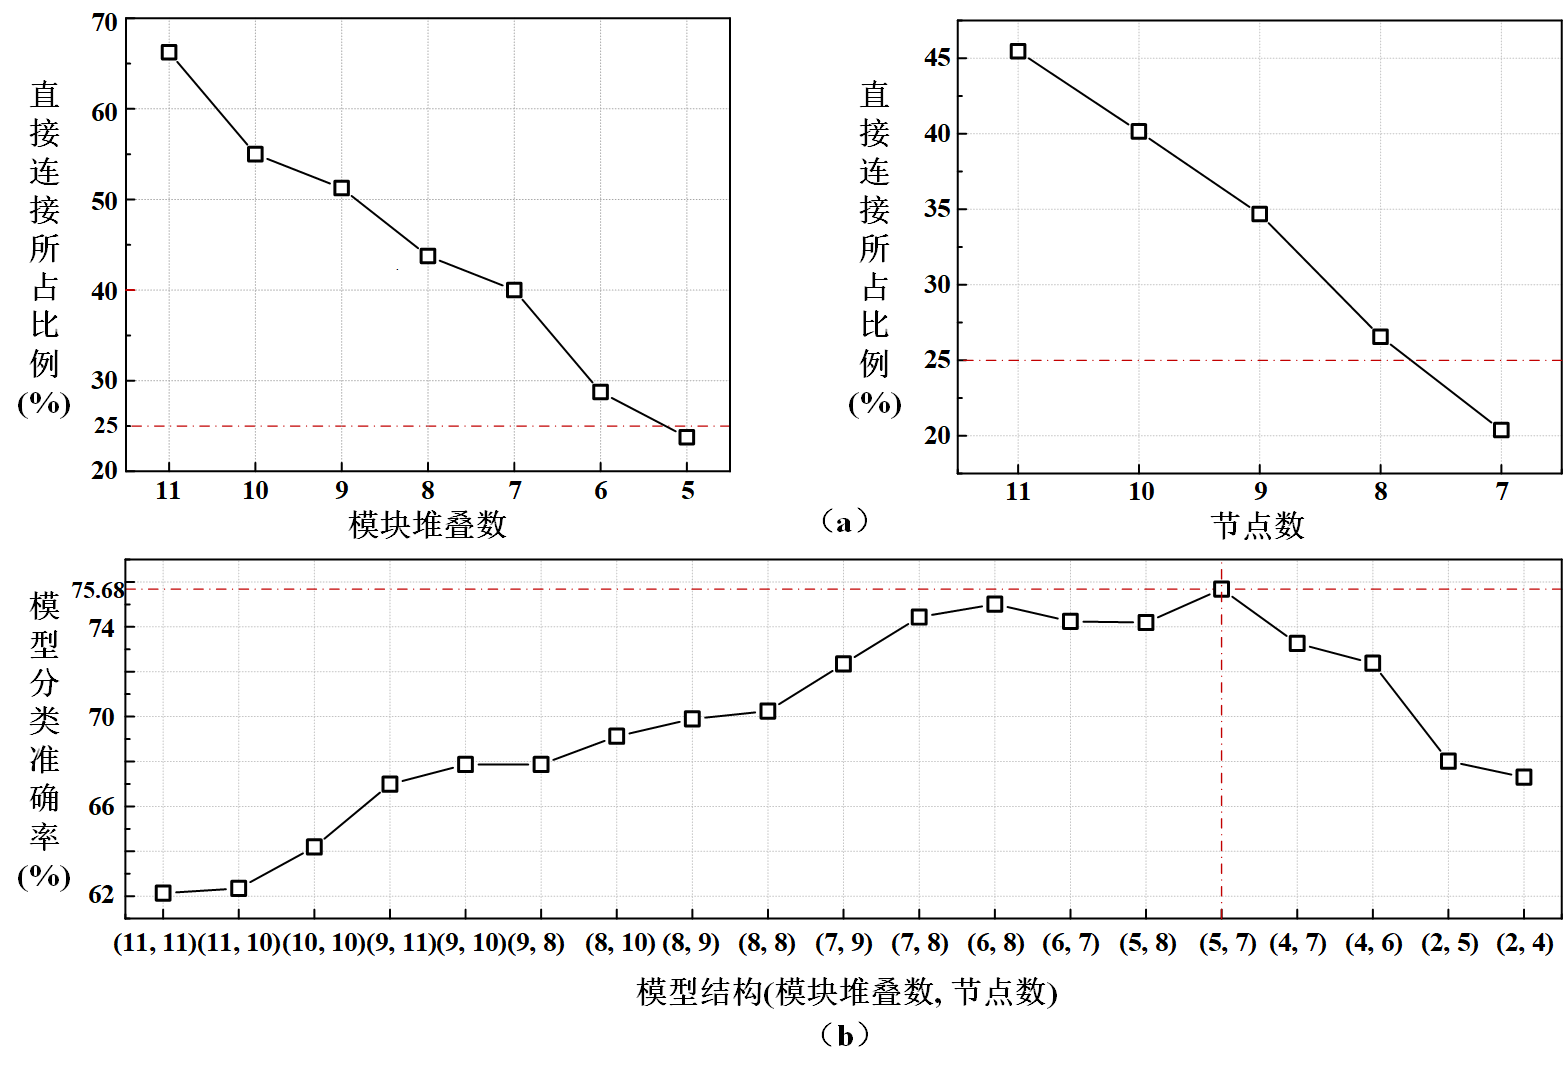
\includegraphics[width=0.60\textheight]{SEED消融.png}
	\caption{SEED数据集网络搜索进程} 
	\label{fig3-3}
\end{figure}


\begin{figure}[!b]
	\centering
	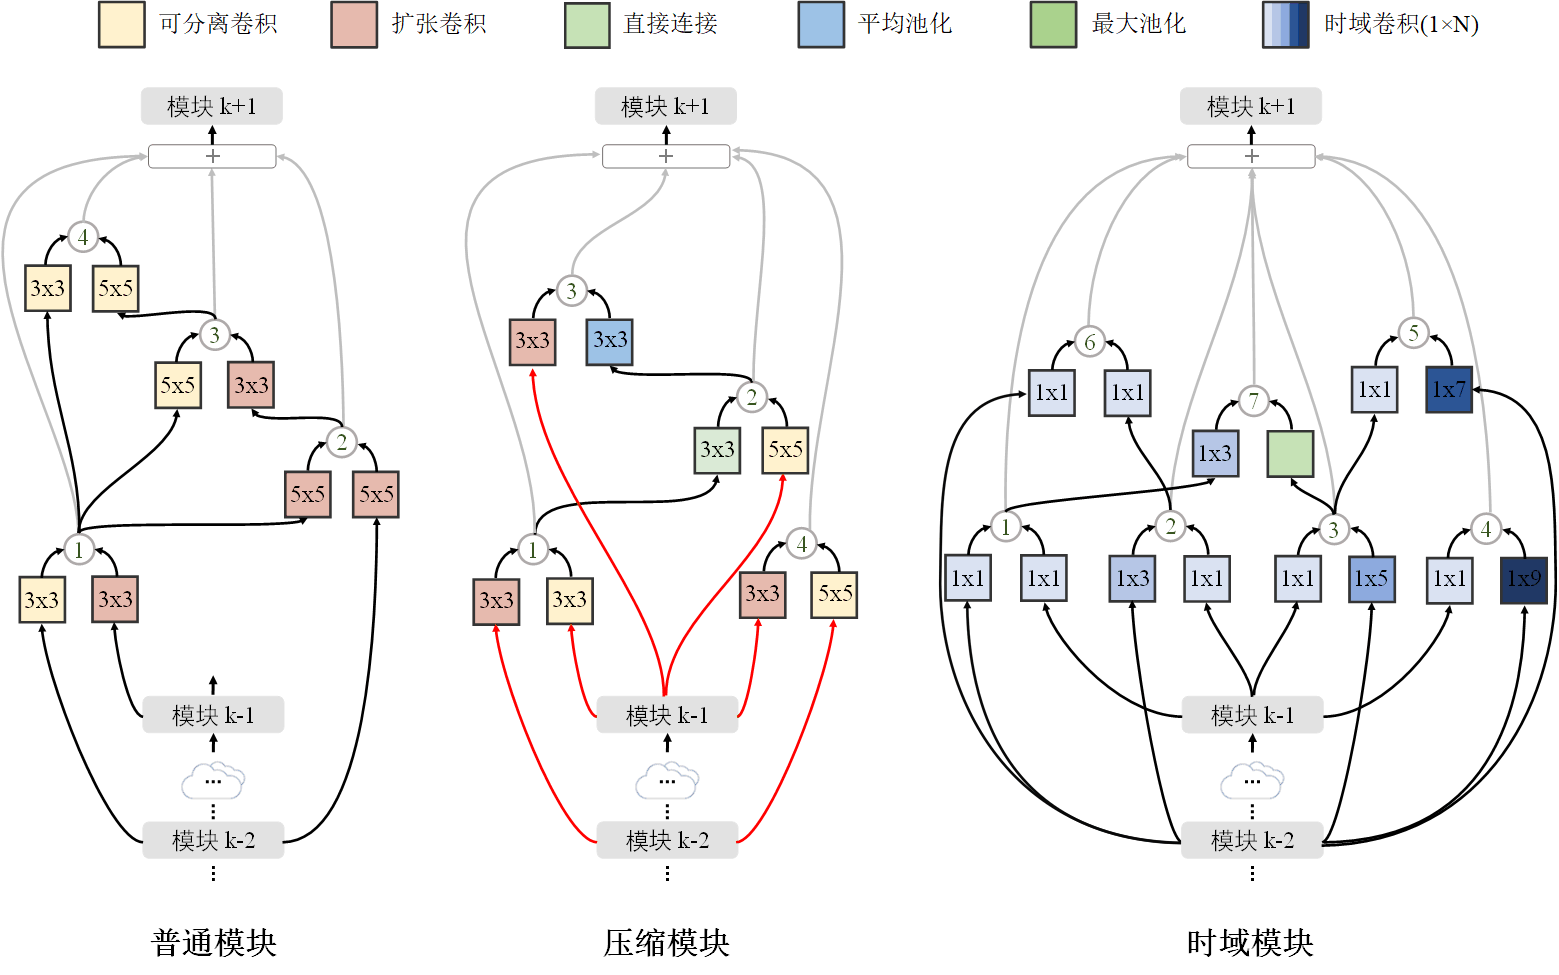
\includegraphics[width=0.61\textheight]{SEED模块.png}
	\caption{SEED数据集上搜索到的三种模块结构} 
	\label{fig3-4}
\end{figure}


\begin{table*}[!h]
\caption{SEED数据集上获得的CNN架构的详细参数}  \label{tab3-2}
\centering
\wuhao{
    \begin{threeparttable}
    \setlength{\tabcolsep}{3mm}{
        \begin{tabular}{cccc}
            \toprule
            \textbf{模块}   &  \textbf{节点} &  \textbf{输入}   &  \textbf{选取的操作}\\ 
            \midrule
            
            \multirow{4}*{普通模块} &节点1     &$concat$(模块k-2,模块k-1)   &3×3可分离卷积,3×3扩张卷积    \\
                                   &节点2     &$concat$(模块k-2,节点1)   &5×5扩张卷积,5×5扩张卷积    \\
                                   &节点3     &$concat$(节点1,节点2)   &5×5可分离卷积,3×3扩张卷积    \\
                                   &节点4     &$concat$(节点1,节点3)   &3×3可分离卷积,5×5可分离卷积    \\
            \midrule
            \multirow{4}*{压缩模块} &节点1     &$concat$(模块k-2,模块k-1)   &3×3扩张卷积,3×3可分离卷积    \\
                                   &节点2     &$concat$(模块k-1,节点1)   &5×5可分离卷积,3×3最大池化    \\
                                   &节点3     &$concat$(模块k-1,节点2)   &3×3扩张卷积,3×3平均池化    \\
                                   &节点4     &$concat$(模块k-2,模块k-1)   &5×5可分离卷积,3×3扩张卷积    \\
            \midrule
            \multirow{7}*{时域模块} &节点1     &$concat$(模块k-2,模块k-1)   &1×1时域卷积,1×1时域卷积    \\
                                   &节点2     &$concat$(模块k-2,模块k-1)   &1×3时域卷积,1×1时域卷积    \\
                                   &节点3     &$concat$(模块k-2,模块k-1)   &1×5时域卷积,1×1时域卷积    \\
                                   &节点4     &$concat$(模块k-2,模块k-1)   &1×9时域卷积,1×1时域卷积    \\
                                   &节点5     &$concat$(模块k-2,节点3)   &1×7时域卷积,1×1时域卷积    \\
                                   &节点6     &$concat$(模块k-2,节点2)   &1×1时域卷积,1×1时域卷积    \\
                                   &节点7     &$concat$(节点1,节点3)   &1×3时域卷积,直接连接    \\
            \bottomrule
        \end{tabular}
        }
        \begin{tablenotes}
	    \footnotesize
	    \item $concat$: 指串联操作(concatenate)。
    \end{tablenotes}
    \end{threeparttable}
    }
\end{table*}




(2) 分类结果

表\ref{tab3-3}给出了所提出的模型和对比算法在SEED数据集上的分类结果。所有的方法都使用了全部62个通道的数据,并使用LOSO交叉验证方案。作为一个典型的神经网络模型,本节所提出的方法会因为随机种子的变化而产生不同的初始化结果,影响模型的最终分类性能。经过多次试验,本模型在SEED数据集上的平均分类精度分布在0.81到0.84之间。在表\ref{tab3-3}中,给出了多次试验后的分类结果中间值。

\begin{table*}[!h]
\caption{SEED数据集不同频段的分类结果(平均值\%/标准差)以及模型复杂度}  \label{tab3-3}
\centering
\wuhao{
    \begin{threeparttable}
    \setlength{\tabcolsep}{0.20mm}{
        \begin{tabular}{cccccccc}
            \toprule
            \multirow{2}*{\textbf{模型}}   &  \multirow{2}*{\textbf{$\delta$}\textbf{频段}} &  \multirow{2}*{\textbf{$\theta$}\textbf{频段}}   & \multirow{2}*{ \textbf{$\alpha$}\textbf{频段}} & \multirow{2}*{\textbf{$\beta$}\textbf{频段}} &  \multirow{2}*{\textbf{$\gamma$}\textbf{频段}} &  \multirow{2}*{\textbf{全频段}} &  \textbf{模型复杂度}\\ 
            &&&&&& &\textbf{参数量(M)}\\
            \midrule          
            TCA\cite{3-19} &44.10/8.22     &41.26/9.21   &42.93/14.33 &43.93/10.06 &48.43/9.73 &63.64/14.88 &$\mathrm{O}\left(\mathrm{n}^2 \mathrm{~d}\right)$     \\
            DANN\cite{3-20} &-     &-   &- &- &- &75.08/11.18 &0.2573     \\
            Cimtay等人\cite{3-21} &-     &-   &- &- &- &78.34 &-     \\
            Fdez等人\cite{3-22} &-     &-   &- &- &- &79.60/10.40 &0.0250     \\
            DGCNN\cite{3-23} &49.79/10.94     &46.36/12.06   &48.29/12.28 &56.15/14.01 &54.87/17.53 &79.95/9.02 &-     \\
            ASFM\cite{3-24} &-     &-   &- &- &- &80.46/6.84 &-     \\
            LF+BiLSTM\cite{3-25} &-    &-   &- &- &- &81.04/6.88 &-     \\
            CNN-DDC\cite{3-26} &-     &-   &- &- &- &82.16/4.43 &-     \\
            BiDANN-S\cite{3-27} &63.01/7.49     &63.22/7.52   &63.50/9.50 &73.59/9.12 &73.72/8.67 &84.14/6.87 & -    \\
            RGNN\cite{3-28} &64.88/6.87     &60.69/5.79   &60.84/7.57 &74.96/8.94 &77.50/8.10 &85.30/6.72 &0.4468     \\
            本章模型 &59.70/13.50     &62.37/7.32   &67.85/8.27 &71.85/8.02 &73.04/ 6.33 &82.96/ 7.85 &0.3795     \\
            \midrule
            频域流     &59.81/ 13.61   &62.08/7.41 &67.96/8.55 &70.32/7.99 &72.65/6.28 &81.82/ 7.96 & 0.2054    \\
            时域流     &-    &-   &- &- &- &48.35/ 6.96 &0.0890     \\
        
            \bottomrule
        \end{tabular}
        }
        \begin{tablenotes}
	    \footnotesize
	    \item -: 模型不具有或未公开相应细节。
    \end{tablenotes}
    \end{threeparttable}
    }
\end{table*}

在单个频段的对比中,本节将输入特征从五个频段更换为单一频段,同时微调模型的输入节点以适应输入维度的变化。对于单个频段,本章所提出的模型在$\alpha$频段取得了所有方法中最高的分类精度;在$\theta$频段也取得了第二高的结果;并且在$\gamma$频段同样具有竞争力。在全部频段上,本章的模型取得了第三高的分类准确率,同时具有可接受的标准差。从准确率的角度来看,本方法在单一频段极具竞争力,在全频段接近于最先进的对比模型,并且优于大多数模型。虽然总体准确率低于RGNN和BiDANN-S,但本方法避免了模型设计过程,在不同的数据集上拥有更好的泛化性能。在SEED数据集上,本章模型的MF1分数为0.8247,AUC值为0.9224。高兴、悲伤和中性三个类别的F1分数分别为0.8287、0.8231和0.8164。从F1分数的角度看,搜索得到的CNN模型对三种不同的情绪类别具有相似的分类能力,对高兴情绪的识别精度最高。从参数规模来看,DANN、RGNN和本章模型具有相同的数量级,但本模型能够取得比DANN更好的判别精度。另一方面,虽然准确率低于RGNN,但本模型的参数数也少于RGNN。Fdez等人提出的模型\cite{3-22}参数数量比其他方法少得多,但需要进行复杂的特征预处理过程才能达到最佳性能。所有的结果都表明,本章所提出的模型对情感分类任务是有效的。

(3) 消融实验

在消融实验中,为了证明当前网络结构的合理性,分别在只有时域流或频域流的搜索空间中搜索网络结构,其分类准确率在表\ref{tab3-3}中给出。如表所示,无论去除哪一部分,模型的最终分类性能都会下降,尤其是去除频域流后。可以看出,时域流在引入了一定数量的参数的同时,对分类精度的提升并不显著,但这一结构的存在是必要的,原因如下。首先,近年来,大量的研究人员致力于探索针对SEED数据集的算法,这使得不同算法之间的竞争非常激烈。从表\ref{tab3-3}中可知,不同算法之间往往只有1\%的性能差异,因此时域流带来的模型性能改进是值得保留的。其次,从表\ref{tab3-4}可以看出,时域流引入的参数数量比频域流少得多,对前向传播时间的影响也极其有限。从本质上讲,时域流带来的参数增加主要来自于模型末端的两个全连接层的变化,而时域流本身并没有引入过多的参数。同时,模型的前向传播时间主要取决于输入数据的维度,而时域流带来的模型复杂度的增加对前向传播时间的影响很小。此外,时域流的影响主要作用在搜索成本增加,即搜索模型架构的时间增长。一旦网络架构被确定,这种影响就会变得非常小,即一旦搜索到网络的最佳架构,本章算法的复杂度不会对使用者产生实质性影响。因此,保留时域流是值得的。本章的方法在Pytorch环境中实现,使用AMD CPU(R9-3950X,3.50 GHz)和NVIDIA GPU(RTX 3090)。
\begin{table*}[!h]
\caption{不同结构模型的时间复杂度}  \label{tab3-4}
\centering
\wuhao{
    \begin{threeparttable}
    \setlength{\tabcolsep}{1.3mm}{
        \begin{tabular}{cccccccccc}
            \toprule
            \multirow{2}*{\textbf{架构类型}}   & \multicolumn{3}{c}{\textbf{SEED}}  & \multicolumn{3}{c}{\textbf{JS-MI}} & \multicolumn{3}{c}{\textbf{疲劳}}\\ 
            &  \textbf{双流} &  \textbf{时域流}   &  \textbf{频域流} &  \textbf{双流} &  \textbf{时域流}   &  \textbf{频域流} &  \textbf{双流} &  \textbf{时域流} &  \textbf{频域流}\\ 
            \midrule          
            搜索耗时 &\multirow{2}*{17.52}     &\multirow{2}*{4.24}   &\multirow{2}*{13.15} &\multirow{2}*{14.47} &\multirow{2}*{3.83} &\multirow{2}*{10.25} &\multirow{2}*{11.67} &\multirow{2}*{2.61} &\multirow{2}*{8.74}\\
            (GPU-hours)&&&&&&&&& \\
            前向传播时间 &\multirow{2}*{2.8765}     &\multirow{2}*{0.7017}   &\multirow{2}*{1.9375} &\multirow{2}*{3.7456} &\multirow{2}*{2.4526} &\multirow{2}*{1.0265} &\multirow{2}*{0.0190} &\multirow{2}*{0.0080} &\multirow{2}*{0.0070}\\
            (Second)&&&&&&&&& \\     
            \bottomrule
        \end{tabular}
        }
    \end{threeparttable}
    }
\end{table*}


\subsection{疲劳驾驶检测公开数据集分类结果}
(1) 结构搜索进程

在疲劳辨识数据集上,使用NAS算法成功获得了相应的CNN架构。与SEED数据集不同,基于疲劳驾驶检测数据集的CNN架构更加简化。从图\ref{fig3-5}中可以看出,在频域流中的模块堆叠数到达两个,时域流中的内部节点数到达四个之前,网络一直处于过拟合状态,算法始终倾向于在两个流中使用弱参数操作。图\ref{fig3-6}给出了NAS过程得到的最终疲劳辨识CNN架构,具体的网络架构在表\ref{tab3-5}中给出。由于最终得到的频域流中模块堆叠数为2,根据堆叠原则,频域流仅包含普通模块,没有压缩模块。

\begin{table*}[!h]
\caption{疲劳驾驶检测数据集上获得的CNN架构的详细参数}  \label{tab3-5}
\centering
\wuhao{
    \begin{threeparttable}
    \setlength{\tabcolsep}{3mm}{
        \begin{tabular}{cccc}
            \toprule
            \textbf{模块}   &  \textbf{节点} &  \textbf{输入}   &  \textbf{选取的操作}\\ 
            \midrule
            
            \multirow{4}*{普通模块} &节点1     &$concat$(模块k-2,模块k-1)   &5×5可分离卷积,直接连接   \\
                                   &节点2     &$concat$(模块k-2,节点1)   &5×5可分离卷积,3×3扩张卷积    \\
                                   &节点3     &$concat$(模块k-2,节点1)   &5×5可分离卷积,直接连接    \\
                                   &节点4     &$concat$(模块k-2,节点2)   &5×5可分离卷积,3×3可分离卷积    \\
    
            \midrule
            \multirow{4}*{时域模块} &节点1     &$concat$(模块k-2,模块k-1)   &1×5时域卷积,1×5时域卷积    \\
                                   &节点2     &$concat$(模块k-2,模块k-1)   &1×5时域卷积,1×7时域卷积    \\
                                   &节点3     &$concat$(模块k-2,模块k-1)   &1×5时域卷积,1×5时域卷积    \\
                                   &节点4     &$concat$(模块k-1,节点1)   &1×1时域卷积,直接连接    \\
            \bottomrule
        \end{tabular}
        }
        \begin{tablenotes}
	    \footnotesize
	    \item $concat$: 指串联操作(concatenate)。
    \end{tablenotes}
    \end{threeparttable}
    }
\end{table*}

同样,为了证明早停算法的有效性,分别比较了重新训练前不同深度模型的验证集分类结果,结果如图\ref{fig3-5}(b)所示。在图中,验证集的准确率不断增加,在当前的网络结构下达到一个峰值。此外,当网络从当前的最佳结构进一步开始简化后,训练集的准确率开始下降,模型表征能力开始不足。

\begin{figure}[!h]
	\centering
	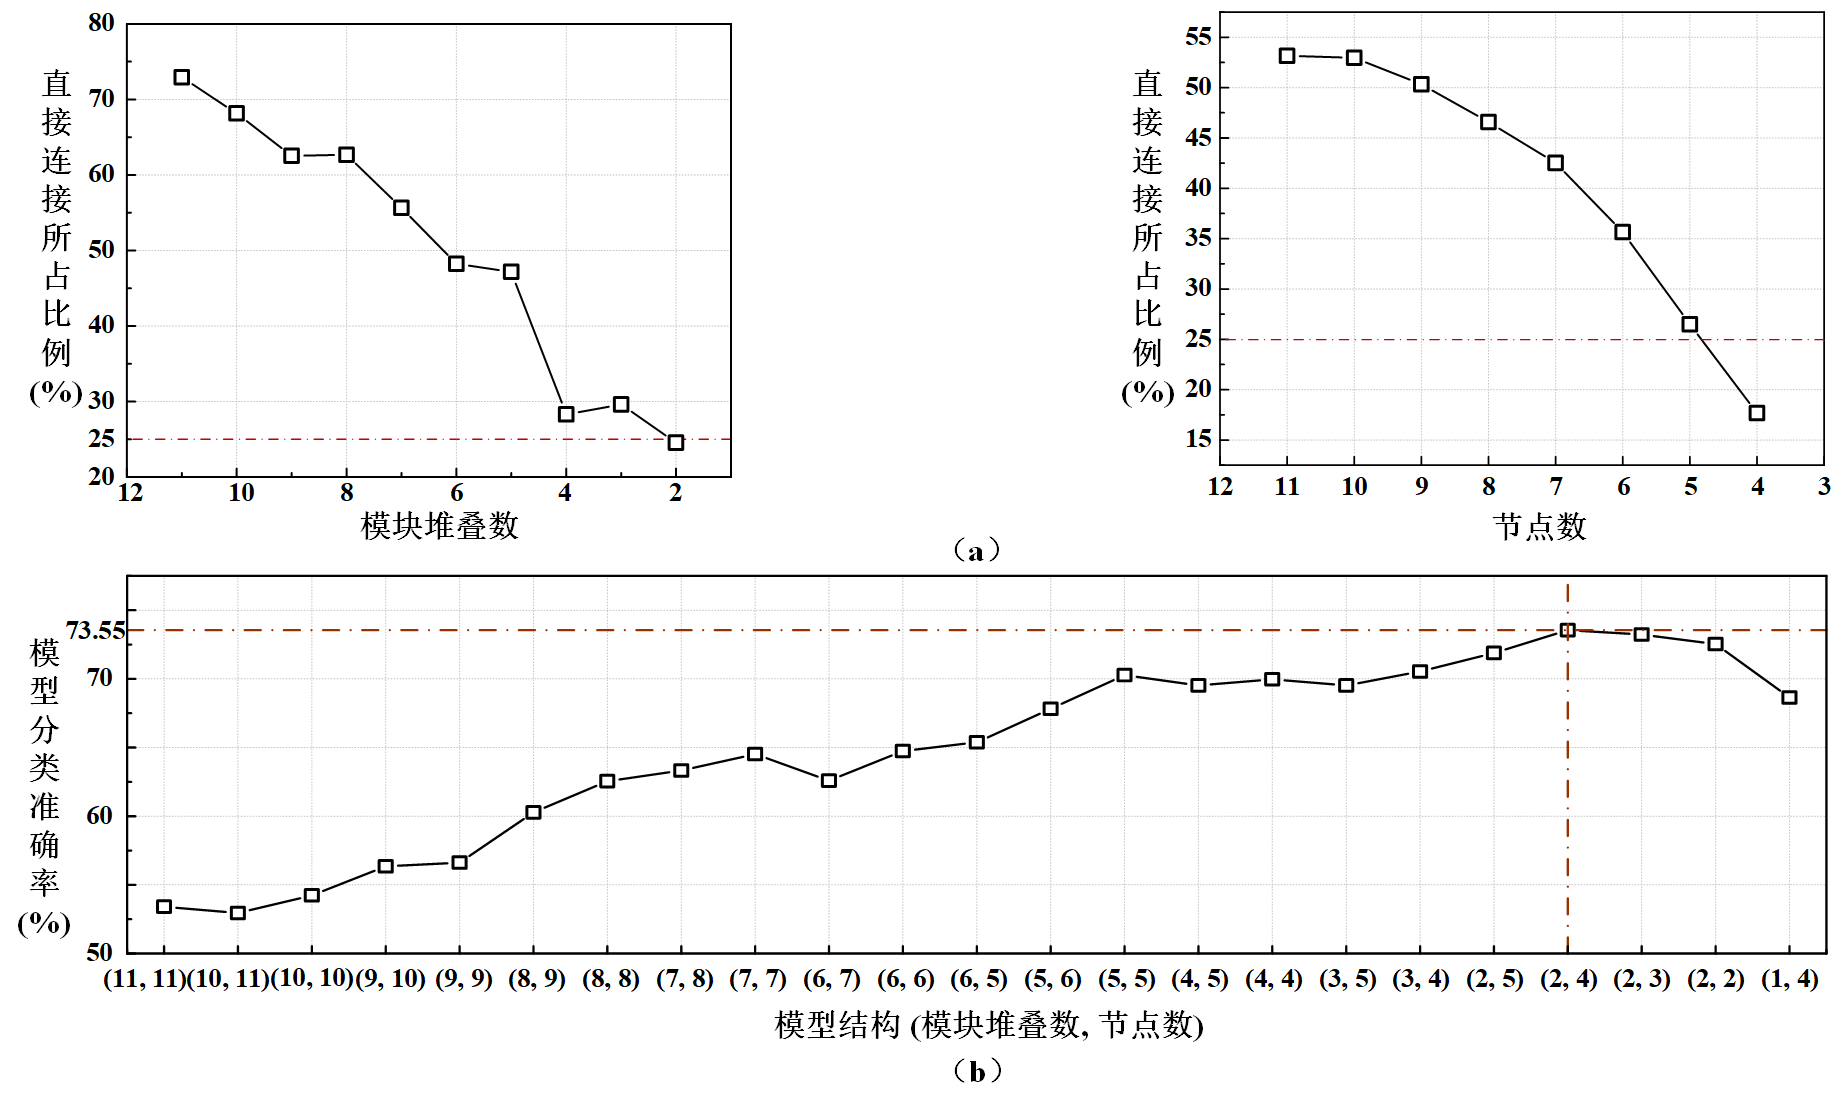
\includegraphics[width=0.60\textheight]{疲劳消融.png}
	\caption{疲劳驾驶检测数据集网络搜索进程} 
	\label{fig3-5}
\end{figure}

\begin{figure}[!h]
	\centering
	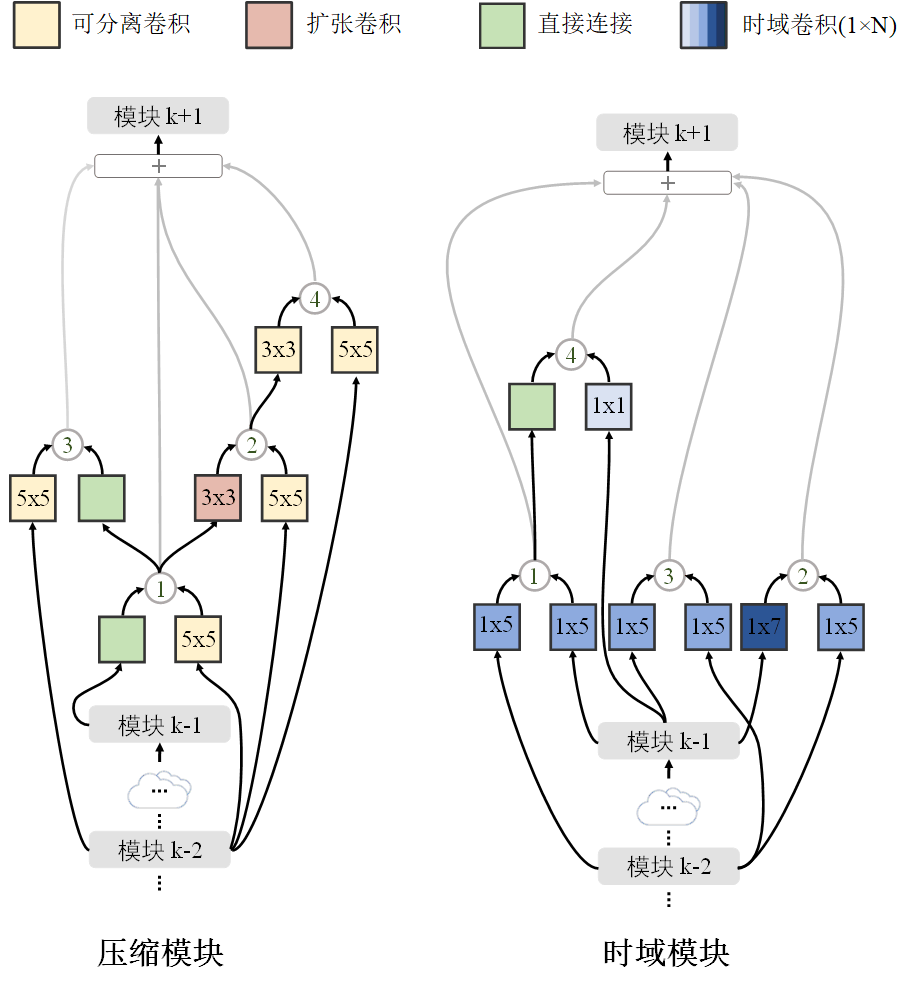
\includegraphics[width=0.40\textheight]{疲劳模块.png}
	\caption{疲劳驾驶检测数据集上搜索到的两种模块结构} 
	\label{fig3-6}
\end{figure}


(2) 分类结果 

由表\ref{tab3-6}可以看到,通过搜索得到的结构能够达到很好的分类效果,其在21个被试上的平均准确率为84.63\%,标准差为7.79。每个被试的准确率如图\ref{fig3-7}所示。表\ref{tab3-6}给出了所提出的模型架构和其他一些基于相同数据集的算法的分类结果,包括每种算法的分类准确率和被试间的标准差。由于标签获取方法的不同,每个算法所使用的数据集会略有不同。为了保证比较的公平性,所有的方法都将基于本文中的数据集进行复现,并使用LOSO交叉验证方案。如前文所述,为了减少随机种子带来的影响,表\ref{tab3-6}的结果是多次运行结果的中间值。值得注意的是,与同样基于EEG图像的算法\cite{3-32}相比,基于NAS算法得到的CNN架构能够达到比人工设计的CNN架构更好的识别精度,这证明了NAS根据当前数据和特征自动设计最佳网络架构时的高度优越性。表\ref{tab3-6}中显示的AUC值和MF1得分显示,本章的NAS策略对疲劳状态识别也很有效。从参数数量的角度来看,虽然本章的方法具有较高的模型复杂度,但它的识别精度也远远高于其他方法,所以认为本章的模型具有足够的竞争力。

\begin{table*}[!t]
\caption{疲劳驾驶检测数据集的分类结果(平均值\%/标准差)以及模型复杂度}  \label{tab3-6}
\centering
\wuhao{
    \begin{threeparttable}
    \setlength{\tabcolsep}{4.8mm}{
        \begin{tabular}{ccccc}
            \toprule
            \multirow{2}*{\textbf{模型}}   &  \multirow{2}*{\textbf{MF1}} &  \multirow{2}*{\textbf{AUC}}   &  \multirow{2}*{\textbf{全频段}} &  \textbf{模型复杂度}\\ 
            &&&&\textbf{参数量(M)}\\
            \midrule          
            EEGNet-4,2\cite{4-2} &59.01     &70.37   &61.87/8.41 &0.0049\\
            LR\cite{3-29} &62.53    &69.98  &61.92/8.54 &$\mathrm{O}\left(\mathrm{n} \mathrm{~d}\right)$     \\
            EEGNet-8,2\cite{4-2} &65.47     &74.67   &66.72/12.03 &0.0073\\
            CNN\cite{3-30} &70.11     &79.36   &70.28/9.66 &0.0143 \\
            TCA+LR\cite{3-19} &71.67     &80.71   &73.41/9.77 &$\mathrm{O}\left(\mathrm{n}^2 \mathrm{~d}+\mathrm{nd}\right)$ \\
            HCNN\cite{3-31} &74.35     &85.73   &75.65/9.84 &0.0035 \\
            Single Frame EEG Image\cite{3-32} &76.85    &89.65   &77.52/11.17 &0.0360   \\
            Temporal EEG Image\cite{3-32} &79.96     &90.36   &80.29/10.95 &0.0363 \\
            本章模型 &84.57     &93.47   &84.63/7.79 &0.2032\\
            \midrule
            频域流     &82.93   &91.82 &83.33/ 7.68 &0.0566 \\
            时域流     &68.56    &83.76   &69.91/ 7.23 &0.0611 \\
        
            \bottomrule
        \end{tabular}
        }
    \end{threeparttable}
    }
\end{table*}

(3) 消融实验

消融实验的实现过程与SEED数据集相同。从表\ref{tab3-6}可以看出,单流结构不足以达到与目前双流结构相同的分类精度,这证明了模型设计的合理性。同样,基于EEG图像的频域流获得了与双流网络类似的分类结果。频域流和时域流各自的计算资源消耗比较见表\ref{tab3-4}。在疲劳数据集上,由于输入数据量较小,而且特征的复杂度较低,所以搜索得到的模型参数数量比在SEED数据集上小得多。尽管由于引入了时域流,模型参数的规模增大了两倍,但考虑到模型本身较低的参数量级,依然认为参数数量的增加对模型的性能没有产生根本的影响。引入时域流后,模型搜索时间增加了2倍多,但前向传播时间仍在毫秒量级内,这对现实应用不会产生过量影响。然而,当追求效率和更少的资源消耗时,单独搜索频域流毫无疑问是一个更具竞争力的选择。

\begin{figure}[!h]
	\centering
	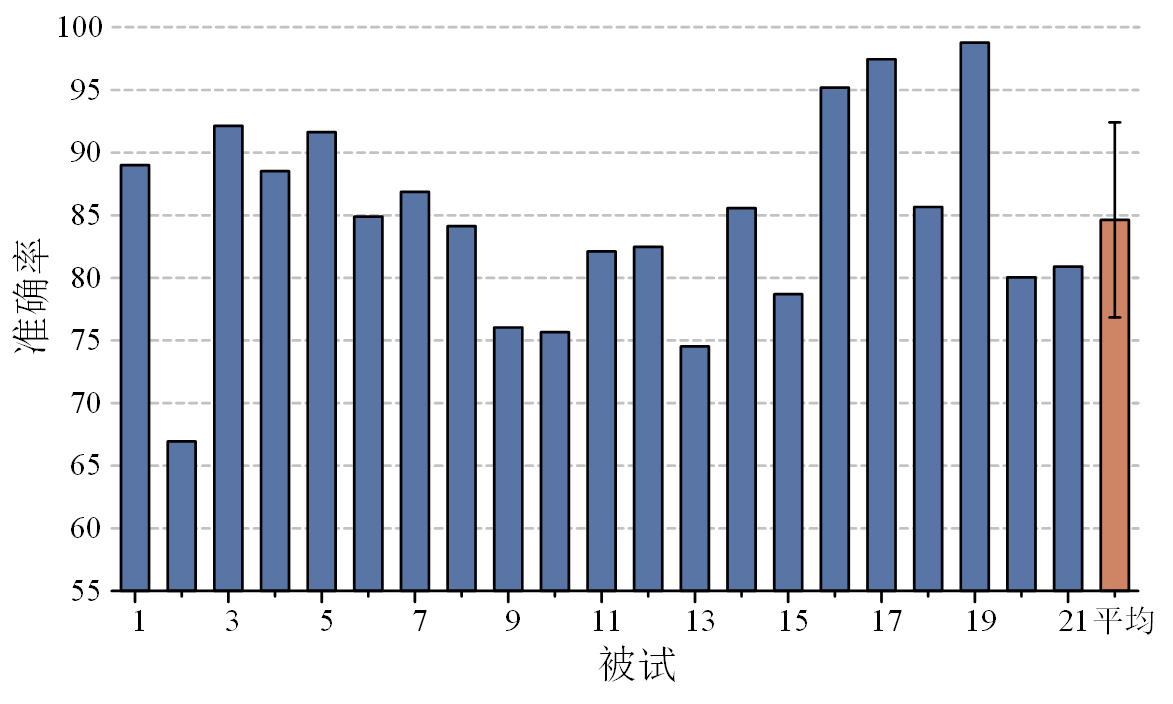
\includegraphics[width=0.45\textheight]{疲劳所有被试.png}
	\caption{疲劳驾驶检测数据集所有被试分类结果} 
	\label{fig3-7}
\end{figure}


\subsection{JS-AINS-40采集的情绪辨识数据集分类结果}

(1) 结构搜索进程

由图\ref{fig3-8}(a)可知,在JS-EM数据集上,直接连接在所有操作中所占的比例依然是判别模型当前拟合状态的有效指标。在直接连接比例低于25\%时,模型获得了在验证集上最优的辨识结果。

\begin{figure}[!h]
	\centering
	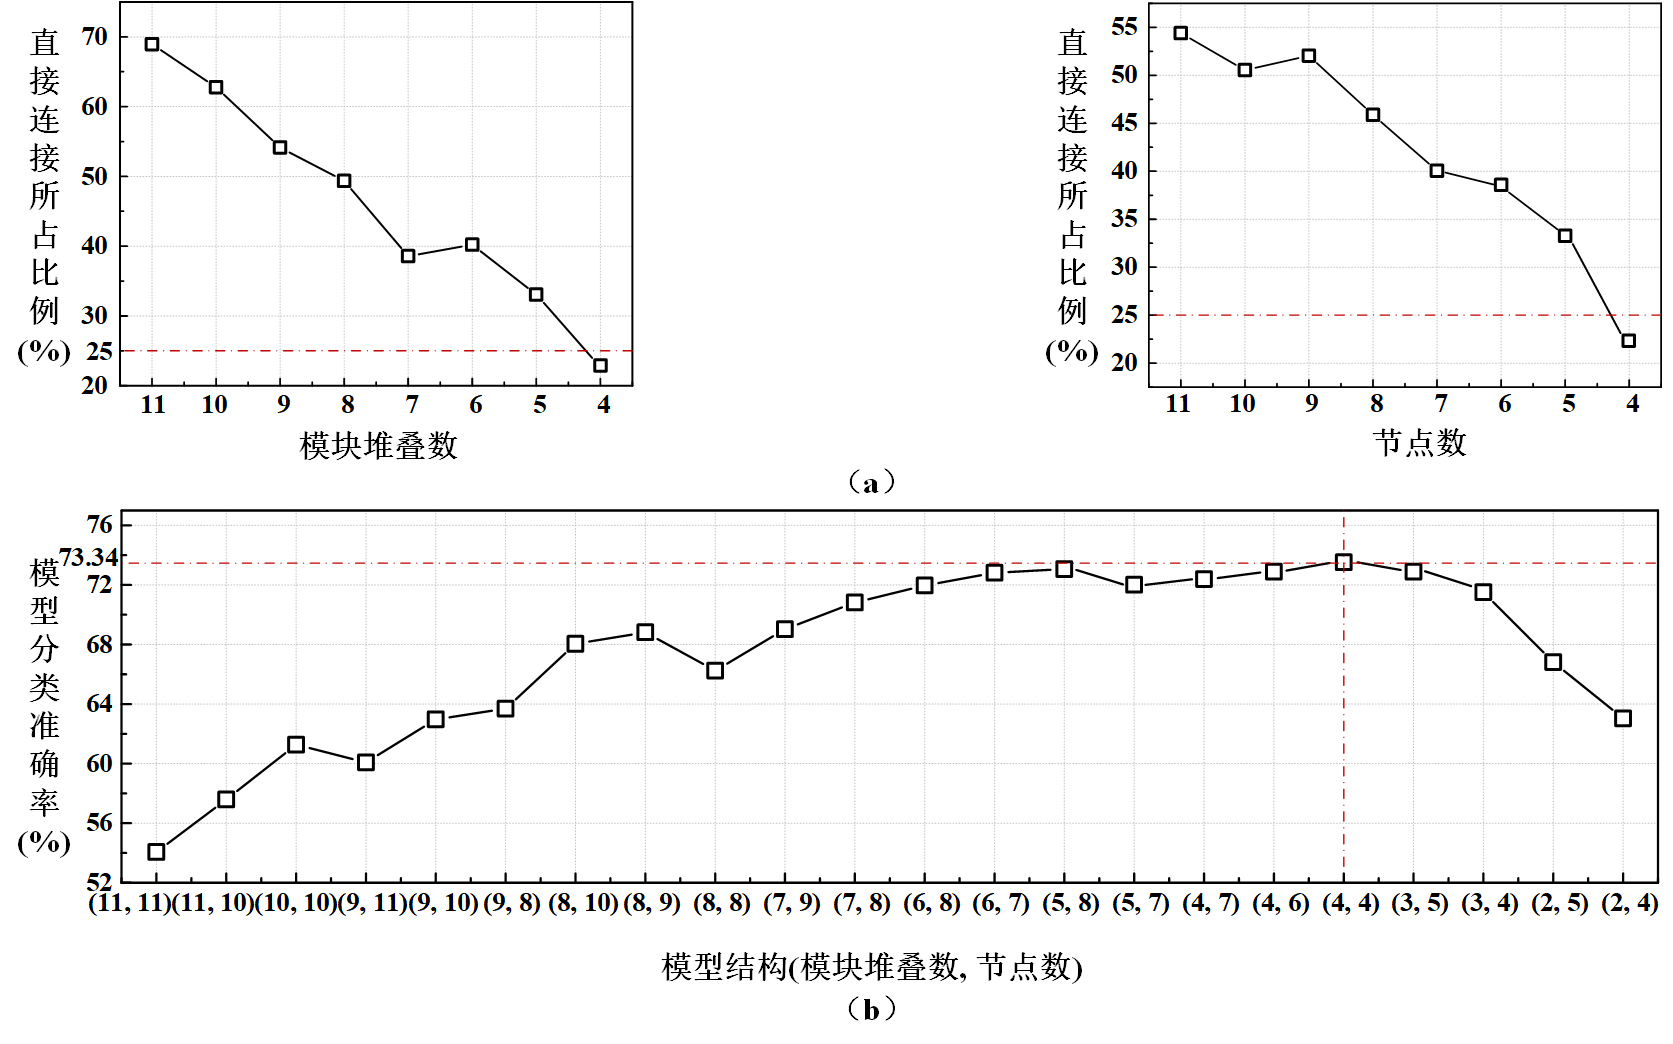
\includegraphics[width=0.60\textheight]{JS-EM消融.png}
	\caption{JS-EM数据集网络搜索进程} 
	\label{fig3-8}
\end{figure}

由于JS-EM数据集所包含的样本量和电极通道数少于SEED数据集,因此模型搜索到的结构也更加简单。由图\ref{fig3-8}(b)可知,在JS-EM数据集上,当频域流堆叠的模块数为4,时域流内部的节点数也为4时,模型在验证集上表现最佳。这证明了搜索得到的模型结构的合理性。各个模块具体的内部结构如图\ref{fig3-9}和表\ref{tab3-8}。由于频域流模块堆叠数量为4,因此其包含普通模块和压缩模块两种单元。

可以看出,早停算法和自适应算法的引入,成功让NAS算法适应了JS-EM数据集。这不仅验证了算法的有效性,也证明了JS-AINS-40系统所采集数据的可靠性。

\begin{figure}[!h]
	\centering
	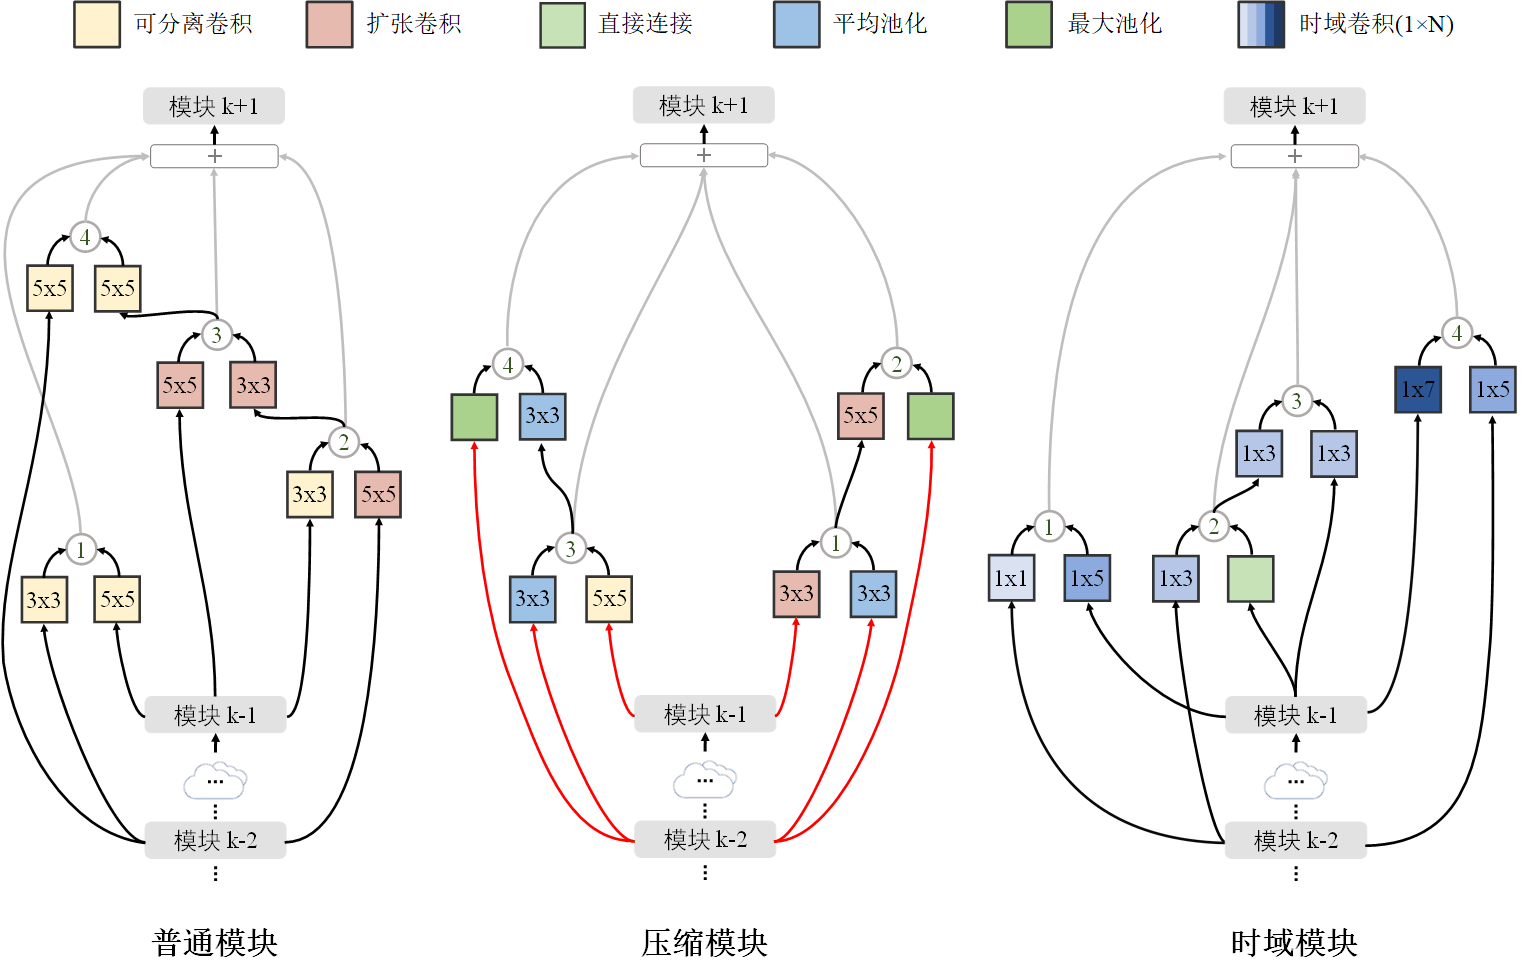
\includegraphics[width=0.60\textheight]{JS-EM模块.png}
	\caption{JS-EM数据集上搜索到的三种模块结构} 
	\label{fig3-9}
\end{figure}

\begin{table*}[!h]
\caption{JS-EM数据集上获得的CNN架构的详细参数}  \label{tab3-8}
\centering
\wuhao{
    \begin{threeparttable}
    \setlength{\tabcolsep}{3mm}{
        \begin{tabular}{cccc}
            \toprule
            \textbf{模块}   &  \textbf{节点} &  \textbf{输入}   &  \textbf{选取的操作}\\ 
            \midrule
            
            \multirow{4}*{普通模块} &节点1     &$concat$(模块k-2,模块k-1)   &3×3可分离卷积,5×5可分离卷积    \\
                                   &节点2     &$concat$(模块k-2,模块k-1)   &5×5扩张卷积,3×3可分离卷积    \\
                                   &节点3     &$concat$(模块k-1,节点2)     &5×5扩张卷积,3×3扩张卷积    \\
                                   &节点4     &$concat$(模块k-2,节点3)     &5×5可分离卷积,5×5可分离卷积    \\
            \midrule
            \multirow{4}*{压缩模块} &节点1     &$concat$(模块k-2,模块k-1)   &3×3平均池化,3×3扩张卷积    \\
                                   &节点2     &$concat$(模块k-2,节点1)     &直接连接,5×5扩张卷积    \\
                                   &节点3     &$concat$(模块k-2,模块k-1)   &3×3平均池化,5×5可分离卷积    \\
                                   &节点4     &$concat$(模块k-2,节点3)     &直接连接,3×3平均池化    \\
            \midrule
            \multirow{4}*{时域模块} &节点1     &$concat$(模块k-2,模块k-1)   &1×1时域卷积,1×5时域卷积    \\
                                   &节点2     &$concat$(模块k-2,模块k-1)   &1×3时域卷积,直接连接    \\
                                   &节点3     &$concat$(模块k-1,节点2)   &1×3时域卷积,1×3时域卷积    \\
                                   &节点4     &$concat$(模块k-2,模块k-1)   &1×5时域卷积,1×7时域卷积    \\
            \bottomrule
        \end{tabular}
        }
        \begin{tablenotes}
	    \footnotesize
	    \item $concat$: 指串联操作(concatenate)。
    \end{tablenotes}
    \end{threeparttable}
    }
\end{table*}


\begin{table*}[!h]
\caption{JS-EM数据集不同频段的分类结果(平均值\%/标准差)以及模型复杂度}  \label{tab3-9}
\centering
\wuhao{
    \begin{threeparttable}
    \setlength{\tabcolsep}{0.15mm}{
        \begin{tabular}{cccccccc}
            \toprule
            \multirow{2}*{\textbf{模型}}   &  \multirow{2}*{\textbf{$\delta$}\textbf{频段}} &  \multirow{2}*{\textbf{$\theta$}\textbf{频段}}   & \multirow{2}*{ \textbf{$\alpha$}\textbf{频段}} & \multirow{2}*{\textbf{$\beta$}\textbf{频段}} &  \multirow{2}*{\textbf{$\gamma$}\textbf{频段}} &  \multirow{2}*{\textbf{全频段}} &  \textbf{模型复杂度}\\
            &&&&&&&\textbf{参数量(M)}\\
            \midrule          
            TCA\cite{3-19} &41.46/8.35     &40.07/9.32   &39.50/11.26 &42.48/11.14 &46.41/8.72 &60.35/13.97 
            
            &$\mathrm{O}\left(\mathrm{n}^2 \mathrm{~d}\right)$     \\
  
  
            DANN\cite{3-20} &-     &-   &- &- &- &71.90/12.41 &0.2216     \\

            
            Fdez等人\cite{3-22}     &-     &-   &- &- &- &75.01/9.94 &0.0194     \\
            
            
            RGNN\cite{3-28}   &62.45/6.54     &60.23/6.08   &60.79/7.68 &71.98/8.11 &72.63/7.95 &80.92/6.67 &0.3951     \\
          
            本章模型           &58.15/13.77     &59.76/7.04   &63.59/8.56 &68.09/7.63 &69.58/6.20 &78.50/7.51 &0.3043     \\
            \midrule
            频域流     &58.04/ 14.32   &59.06/7.89 &63.42/8.43 &68.04/7.85 &68.11/6.37 &77.84/8.18 & 0.1783    \\
            时域流     &-    &-   &- &- &- &42.98/ 7.08 &0.0687     \\
        
            \bottomrule
        \end{tabular}
        }
        \begin{tablenotes}
	    \footnotesize
	    \item -: 模型不具有相应细节。
    \end{tablenotes}
    \end{threeparttable}
    }
\end{table*}

(2) 分类结果 

本章所提出算法的最终分类结果如表\ref{tab3-9}所示。本节选取了表\ref{tab3-3}中开源的对比方法对JS-EM数据集进行了评估,同时对比所提出算法的性能。由于本节的主要目的不在于验证算法的有效性,而是检验不同算法能否正确辨识JS-EM数据集,即JS-AINS-40系统采集的情绪EEG数据是否能够用来辨识人脑情绪状态。因此,这里仅引入了四种不同的对比方法。从结果可知,基于传统机器学习的情绪辨识算法、基于对抗学习的辨识方法以及基于图卷积的分类模型均在JS-EM数据集上获得了成功。这证明了JS-EM数据集的可靠性,并进一步验证了JS-AINS-40系统的稳定性。

在JS-EM数据集上,本章所提出模型的MF1分数为0.7992,AUC值为0.8807。高兴,悲伤,中性三个类别对应的F1分数分别为0.8011,0.7906,0.7858。模型依然对三种类别具有相近的分类能力,并且对高兴的辨识精度最高。

尽管在所有方法中,RGNN依然取得了最佳的分类结果,但是本章算法也仍然具有足够的竞争力,并且本章算法具有更低的模型空间复杂度。同样的,无需人工进行模型结构设计,依然是本章算法的最大优势。与表\ref{tab3-3}对比可知,所有方法在JS-EM数据集上的结果均低于SEED数据集。这主要源自于JS-EM数据集较少的通道数量和样本量,让算法更难以提取到足够具有辨识性的特征。但毫无疑问,JS-EM数据集上的结果依然处于可接受范围,这证明了JS-ANIS-40系统具备足够的可靠性。

(3) 消融实验

本节进行的消融实验,其具体内容与之前的数据集相同。在表\ref{tab3-9}中给出了单流结构的分类准确率,相应的时间消耗可以见表\ref{tab3-4}。可以看到,频域流在模型中依然占据主要作用。但是,在JS-EM数据集上,时域流的作用有所降低,添加时域流后,模型的准确率仅上升了不到0.7\%。这可能是由于本章使用了JS-EM数据集中全部40通道的EEG数据,模型没有直接获取关键特征,导致时域特征提供的帮助更为有限。然而,时域流的引入毫无疑问让模型的辨识能力获得了提升,并进一步降低了不同被试间结果的标准差,这证明了时域流的存在具有必要性。

虽然JS-EM数据集采用了与SEED相似的实验流程设计,但是由于被试人数,试验次数,EEG通道数等众多因素的影响,二者的最优模型结构仍具有较大的差异。这也进一步导致了基于二者的模型在空间复杂度(参数量)与时间复杂度(前向传播时间)上的差异。从结果可以看出,所提出算法在JS-EM数据集上同样具备足够的泛化性能。


\subsection{与其他NAS算法的比较}

在表\ref{tab3-7}中,除了RL-NAS\cite{3-33}之外,所有的模型都不能在未进行调整时在EEG数据上获得足够的分类精度(堆叠模块数量均被设定为8时)。这从另一个角度验证了本章对PC-DARTS改进的合理性。由于Robustified DARTS\cite{3-36}引入了更强的L2正则化和早停策略,这使得它在模型复杂度较高时取得了比PC-DARTS更好的结果。另一方面,RL-NAS不需要进行结构调整,因为这一模型结构是面向EEG信号而设计的。

\begin{table*}[!h]
\caption{不同NAS算法在疲劳驾驶检测数据集上的LOSO分类结果(平均值\%/标准差)}  \label{tab3-7}
\centering
\wuhao{
    \begin{threeparttable}
    \setlength{\tabcolsep}{4.1mm}{
        \begin{tabular}{ccc}
            \toprule
            \textbf{模型}   &  \textbf{未进行调整时的分类准确率} & \textbf{进行调整后的分类准确率} \\ 
            \midrule          
            RL-NAS\cite{3-33} &71.59/7.37     &71.59/7.37 \\
            DARTS\cite{3-34} &58.14/6.76     &76.54/8.02 \\
            SNAS\cite{3-35} &57.59/6.53    &77.41/7.90  \\
            Robustified DARTS\cite{3-36} &64.20/6.44     &82.57/7.53 \\
            本章模型 &62.58/6.37     &83.33/7.68   \\
        
            \bottomrule
        \end{tabular}
        }
    \end{threeparttable}
    }
\end{table*}

除了RL-NAS之外,所有NAS搜索算法的基础模型架构都过于复杂,在疲劳的数据集上会造成严重的过拟合问题,最终导致分类结果不佳。在此基础上进行比较是没有意义的。由于参与比较的模型都使用了与DARTS类似的架构,本节借用了本章中搜索得到的最佳网络结构——将对比模型中的堆叠模块数设置为2(除了RL-NAS),并在此基础上进行网络结构搜索。同时,使用EEG时间序列作为RL-NAS模型的输入,其余的对比模型都用EEG图像作为输入。

从表\ref{tab3-7}的最终结果可以看出,RL-NAS取得的分类精度与时域流接近,这是由于时域流的设计思路与RL-NAS相似,两者的模型结构也非常接近。然而,由于RL-NAS中的粒子群优化算法可以微调卷积操作的卷积核个数,使网络的性能得到了更多的提升——因此时域流的精度相对较低。但是,如果参考RL-NAS在本文的搜索空间中加入具有不同卷积核数量的卷积操作,将会导致搜索空间维度激增,带来搜索时间的大幅增加。考虑到这一改动将会带来的计算资源消耗,本章没有采用这一策略。

DARTS和SNAS都发表于2019年,依靠不同的算法进行网络架构搜索,但性能相似,因此取得了类似的分类结果。然而,由于两者都没有约束网络中弱参数操作的选取,因此在EEG上的性能并不理想。Robustified DARTS从不同的角度对NAS的崩塌进行了优化,增加了早停机制和针对“内部目标”的L2正则化系数,从而使分类结果优于DARTS和SNAS。然而,由于本章模型在PC-DARTS的边缘正则化算法基础上引入了针对性的改动,从而使其能够更好地应对NAS的崩塌现象,并在当前的数据集上取得较好的分类精度。同时,PC-DARTS的部分通道采样功能有效地减少了NAS过程中使用的显存大小,为本章的后续改进提供了关键性保障。

综上所述,对于当前的EEG辨识任务来说,本章提出的模型是足够先进的、具有竞争力的。

\section{本章小结}

本章在现有NAS技术基础上改进得到了一个新的模型,以获得基于EEG识别人脑生理状态的CNN框架。这是NAS技术在EEG信号辨识领域的一个创新应用。为了实现将基于图像的NAS技术向EEG时序信号的迁移,本章创新性地设计了一个基于先验知识的有限但合理的搜索空间。同时,为了找到合适的网络深度,降低崩塌的风险,本章引入了层数自适应机制和早停机制。在本章中,时域流被用来提取通道的时间依赖性和通道的具体特征,而频域流则更关注通道的相对位置及其频域特征。该模型的有效性在三个不同的EEG状态评估任务中被分别验证。结果表明,由NAS算法得到的CNN框架能够在情绪识别任务中取得具有竞争力的分类精度,并能在疲劳状态辨识任务中取得一定的优势。

上述结果说明,本章所提出的基于梯度自动优化的脑电辨识模型可以根据不同的数据集构建有针对性的网络架构,并具一定的有效性和通用性。因此,本章所提出的方法是NAS技术向EEG分析领域的有效迁移,并有很大潜力为其他类型的分类和预测任务提供高性能的结果。这可以有效降低研究人员的时间成本,促进CNN在更多领域的应用。

同时,在JS-EM数据集上的结果也证明了JS-AINS-40系统具备足够的可靠性。尽管JS-EM数据集在不同情绪分类算法中取得的结果略低于SEED数据集,但是这一差距依然在实验环境以及被试间差异可能导致的偏差区间内。因此,认为JS-AINS-40系统具备辨识人脑情绪状态的能力。






